
%
%Some new control stuff right here at the top.
%

%Toggle nsf format which sucks vs. aas format which is too long. Toggles
%document class, bibliography, and a few things in macros.txt
\newif\ifnsf
\nsftrue %uses the [x] citations, which is pretty much worse than stalin but is short.
%\nsffalse %Uses aastex, which has informative citations but too long




\ifnsf
\documentclass[11pt]{NSF}
\else
\documentclass[11pt,preprint]{aastex}
\fi



%\pagestyle{empty}  % removes page numbers - DO THIS BEFORE SUBMISSION

\usepackage{natbib}
\usepackage{xspace}
\usepackage{amsmath}
\usepackage{amssymb}
\usepackage{revindent}
\usepackage{color}
\usepackage{wrapfig}
\usepackage{hyperref} %, breakurl}
\usepackage[normalem]{ulem} %for sout to strike out text.
%\usepackage{hyperref}
\hypersetup{colorlinks=true}
\hypersetup{linkcolor=blue}
\hypersetup{citecolor=blue}
\hypersetup{urlcolor=blue}
\renewcommand{\sectionautorefname}{\S}

\def\li{\noindent$\bullet$\quad}
\def\kms{\ifmmode{~{\rm km~s^{-1}}}\else{~km s$^{-1}$}\fi}
\def\cc{\ifmmode{~{\rm cm^{-3}}}\else{~cm$^{-3}$}\fi}
\def\fesc{\ifmmode{{f_{esc}}}\else{$f_{\rm esc}$}\fi}
\def\fstar{\ifmmode{{f_\star}}\else{$f_\star$}\fi}
\def\lsim{\lower0.3em\hbox{$\,\buildrel <\over\sim\,$}}
\def\gsim{\lower0.3em\hbox{$\,\buildrel >\over\sim\,$}}
\def\hst{{\it HST}}
\def\otvet{{\sl OTVET}}
\def\enzo{{\sc Enzo}}
\def\moray{{\sc Moray}}
\def\yt{{\sc yt}}
\def\Ms{\ifmmode{~{\rm M_\odot}}\else{M$_\odot$}\fi}
\def\Zs{\ifmmode{~{\rm Z_\odot}}\else{Z$_\odot$}\fi}
\def\h2{H$_2$}
\def\Ol{$\Omega_\Lambda$}
\def\Om{$\Omega_M$}
\def\Ob{$\Omega_b$}
\def\tcool{$t_{\rm{cool}}$}
\def\tcross{$t_{\rm{cross}}$}
\def\tdyn{$t_{\rm{dyn}}$}
\def\tvir{$T_{\rm{vir}}$}
\def\lya{Ly$\alpha$}
\def\hh{H$_2$}
\def\nat{Nature}
\def\apj{ApJ}
\def\aj{AJ}
\def\apjl{ApJL}
\def\apjs{ApJS}
\def\mnras{MNRAS}
\def\araa{ARA\&A}
\def\aap{A\&A}
\def\nar{NewAR}
\def\na{New Astronomy}
\def\rmxaa{Revista Mexicana de Astronomia y Astrofisica}
\def\physrep{Physics Reports}
\def\pasa{Publications of the Astronomical Society of Australia}

\def\sfr{\ensuremath{\Sigma_{\rm{SFR}}}}
\def\sgas{\ensuremath{\Sigma_{\rm{gas}}}}
\def\tdyn{\ensuremath{t_{\rm{dyn}}}}
\def\halpha{\ensuremath{\rm{H}_{\alpha}}}

\newcommand{\hi}{H {\sc i}}
\newcommand{\hii}{H {\sc ii}}
\newcommand\unit[1]{\; \textrm{#1}}
\newcommand\mysec[1]{\noindent\textbf{#1}:}
\def\hr{\begin{center}
  \line(1,0){250}
\end{center}
}

\newcommand{\red}[1]{\textcolor{red}{#1}}
\newcommand{\blue}[1]{\textcolor{blue}{#1}}
\newcommand{\green}[1]{\textcolor{green}{#1}}
\newcommand{\bwo}[1]{\textcolor{red}{(BWO: #1)}}
\newcommand{\dcc}[1]{\textcolor{blue}{(DCC: #1)}}
\newcommand{\thischange}[1]{\textcolor{red}{#1}}


\newcommand{\needcite}[1]{\textcolor{red}{(cite: #1)}}

\newcommand{\note}[1]{{\color{red} \bf #1}}
%\newcommand{\todo}[1]{{\noindent$\bullet$\quad {\color{red} \bf TODO
%      (#1): }}}
\newcommand{\todo}[1]{\reversemarginpar\marginpar{\color{red}\bf TODO}
  {\color{red} \noindent \bf(#1)}}

\newcommand{\dave}{\textcolor{blue}{DAVE DO THIS:   }}
\newcommand{\brian}{\textcolor{red}{BRIAN DO THIS:   }}

%%%%%%%%%%%%%%%%%%%%%%%%%%%%%%%%%%%%%%%%%%%%%%%%%%%%%%%%%%%%%%%%%%%%%%%%
%%%%%%%%%%%%%%%%%%%%%%%%%%%%%%%%%%%%%%%%%%%%%%%%%%%%%%%%%%%%%%%%%%%%%%%%
%%%%%%%%%%%%%%%%%%%%%%%%%%%%%%%%%%%%%%%%%%%%%%%%%%%%%%%%%%%%%%%%%%%%%%%%

%\def\paragraph{\@startsection{paragraph}{4}{\z@}{1.0ex plus 
%    0.25ex minus 0.25ex}{-1em}{\normalsize\bf}}

\let\oldenumerate=\enumerate
\let\endoldenumerate=\endenumerate
\renewenvironment{enumerate}{%
  \begin{oldenumerate}%
    \setlength{\itemsep}{0.0ex}%
    \setlength{\parskip}{0.25ex}%
  }%
  {%
  \end{oldenumerate}%
}

\let\olditemize=\itemize
\let\endolditemize=\enditemize
\renewenvironment{itemize}{%
  \begin{olditemize}%
    \setlength{\itemsep}{0.0ex}%
    \setlength{\parskip}{0.25ex}%
  }%
  {%
  \end{olditemize}%
}

%%%%%%%%%%%%%%%%%%%%%%%%%%%%%%%%%%%%%%%%%%%%%%%%%%
%% Additions from AASTeX
%%%%%%%%%%%%%%%%%%%%%%%%%%%%%%%%%%%%%%%%%%%%%%%%%%
\ifnsf
\newcommand\ion[2]{#1$\;${\small\rmfamily\rm{#2}}\relax}
\def\eps@scaling{1.0}% 
\newcommand\epsscale[1]{\gdef\eps@scaling{#1}}% 
\newcommand\plotone[1]{% 
 \centering 
 \leavevmode 
 \includegraphics[width={\eps@scaling\columnwidth}]{#1}% 
}% 
\newcommand\plottwo[2]{% 
 \centering 
 \leavevmode 
 \columnwidth=.5\columnwidth 
 \includegraphics[width={\eps@scaling\columnwidth}]{#1}% 
 \hfil 
 \includegraphics[width={\eps@scaling\columnwidth}]{#2}% 
}% 
\newcommand{\ssr}{Space~Sci.~Rev.}
\fi




%%%% PUT NEW COMMANDS AND DEFINITIONS HERE %%%%
\usepackage{graphicx, natbib, color, bm, amsmath, epsfig}

%
% Hijacked and hacked from aastex.cls
%
%\def\newblock{\hskip .11em\@plus.33em\@minus.07em}%

%\newcommand\plotone[1]{%
% \typeout{Plotone included the file #1}
% \centering
% \leavevmode
% \includegraphics[width={\eps@scaling\columnwidth}]{#1}%
%}
%\newcommand\plotone[1]{
% \includegraphics[width=3.0in]{#1}%
%}
%\let\tableline=\hline
%enzo commands
\newcommand\jcompphys{J.~Comput.~Phys}
\newcommand\physfluidsa{Phys.~Fluids~A}
\newcommand\physfluids{Phys.~Fluids}
\newcommand\physlettA{Phys.~Lett.~A}
\newcommand\jfm{J.~Fluid~Mech.}
\newcommand\ccm{Comput.~Phys.~Commun.}
\newcommand\jphysique{J.~Physique~I}
\newcommand\revmodphys{Rev.~Mod.~Phys.~}

%\newcommand\aap{\ref@jnl{A\&A}}% 
%\newcommand\prb{\ref@jnl{Phys.~Rev.~B}}% 
          % Physical Review B: Solid State 


\newcommand{\ratio}{\mathcal{R}}
\newcommand{\Lmax}{\ell_{\rm max}}
\newcommand{\menzo}{{EnzoMHD}}
\newcommand{\Menzo}{{EnzoMHD}}
\newcommand{\zeus}{{\small ZEUS}}
\newcommand{\Lbox}{L_{\rm box}}
\newcommand{\Nroot}{N_{\rm root}}
\newcommand{\K}{\,\rm K}
\newcommand{\grid}{{\tt grid}}

%\newcommand{\lct}[3]{\ensuremath{\epsilon_{#1,#2,#3}}}
\newcommand{\lct}[1]{\ensuremath{\epsilon_{#1}}}
%grid location commands.
\newcommand{\iph}{i + \frac{1}{2}}
\newcommand{\imh}{i - \frac{1}{2}}
\newcommand{\jph}{j + \frac{1}{2}}
\newcommand{\jmh}{j - \frac{1}{2}}
\newcommand{\kph}{k + \frac{1}{2}}
\newcommand{\kmh}{k - \frac{1}{2}}

\newcommand{\ipmh}{i \pm \frac{1}{2}}
\newcommand{\half}{\frac{1}{2}}
\newcommand{\quart}{\frac{1}{4}}
\newcommand{\tquart}{\frac{3}{4}}

%physics commands
\newcommand{\avir}{\ensuremath{\alpha_{\rm{vir}}}}
\newcommand{\mach}{\ensuremath{\mathcal{M}}}
\newcommand{\hmag}{\ensuremath{H_{\rm{M}}}}
\newcommand{\alfmach}{\ensuremath{\mathcal{M_{\rm{A}}}}}
\newcommand{\msun}{\ensuremath{\rm{M}_\odot}}
%\newcommand{\msun}{\ensuremath{M_\odot}}
\newcommand{\lsun}{\ensuremath{L_\odot}}
\newcommand{\rsun}{\ensuremath{R_\odot}}
\def\AD{{\rm{AD}}}

%math commands
\def\rms{\ensuremath{\rm{rms}}}
\newcommand{\dbd}[2]{\frac{ \partial #1 }{ \partial #2} }
\newcommand{\ddbd}[2]{\frac{ d #1 }{ d #2} }
\newcommand{\dDbD}[2]{\frac{ \mathrm{D} #1 }{ \mathrm{D} #2} }
\newcommand{\curl}{\nabla \times}
\newcommand{\divb}{\ensuremath{\nabla \cdot {\bvec}}}
\newcommand{\divv}{\ensuremath{\nabla \cdot {\vvec}}}
\newcommand{\divbo}{$\nabla \cdot {\bf B} = 0$}
\newcommand{\intd}[1]{\int_#1^{#1 + \Delta #1} }
\newcommand{\dt}{\Delta t}
\newcommand{\dx}{\Delta x}
\newcommand{\dy}{\Delta y}
\newcommand{\dz}{\Delta z}
\newcommand{\p}[1]{#1^\prime }
\newcommand{\pp}[1]{#1^{\prime \prime} }
\newcommand{\tff}{\ensuremath{t_{\rm{ff}}}}
\newcommand{\kkmin}{\ensuremath{k/k_{\rm{min}}}}
\newcommand{\kmax}{\ensuremath{k_{\rm{max}}}}

%dcc color commands
\definecolor{orange}{rgb}{1.        ,  0.54,  0}
\newcommand{\orange}[1]{\textcolor{orange}{#1}}

\newcommand{\gtt}[1]{\textcolor{green}{{\tt#1}}}
\newcommand{\yellow}[1]{\textcolor{yellow}{#1}}
\definecolor{meta}{rgb}{0.371,0.617,0.625} %cadet blue for
                                           %non-production worthy
                                           % discussion of the work
\newcommand{\meta}[1]{\textcolor{meta}{#1}}
\newcommand{\aake}[1]{\textcolor{blue}{#1}}
\newcommand{\bld}[1]{\mathbf{#1}}

\def\here{\red{YOUGOTHERE}}
%\newcommand{\hilite}[1]{\textcolor{red}{#1}}
%\newcommand{\hilite}[1]{#1}

%\newcommand{\bold}[1]{{\bf #1}}
%the comment maker, dc: the first one will show all comments in green, 
%the second hides them all.
%\newcommand{\dc}[1]{\textcolor{green}{#1}}
\newcommand{\dc}[1]{}
%\newcommand{\dc}[1]{#1}
%\def\bvec{\ensuremath{\vec{B}}}
%\def\vvec{\ensuremath{\vec{v}}}
\def\Bvec{\ensuremath{{\bf B}}}
\def\Jvec{\ensuremath{{\bf J}}}
\def\Avec{\ensuremath{{\bf A}}}
\def\bvec{\ensuremath{{\bf b}}}
\def\vvec{\ensuremath{{\bf v}}}
\def\uvec{\ensuremath{{\bf u}}}
\def\rvec{\ensuremath{{\bf r}}}
\def\xvec{\ensuremath{{\bf x}}}
\def\kvec{\ensuremath{{\bf k}}}
\def\omegavec{\ensuremath{{\bf \Omega}}}
%\newcommand{\BlockOut}[1]{}
\newcommand{\BlockOut}[1]{#1}
\newcommand{\imp}{\ensuremath{\implies}}
\newcommand{\question}[1]{\textcolor{red}{#1}}
\definecolor{pink}{rgb}{1.        ,  0.75294118,  0.79607843}
\definecolor{maroon}{rgb}{0.69019608,  0.18823529,  0.37647059}
\newcommand{\ToRead}[1]{\textcolor{maroon}{#1}}
\newcommand{\ToReadUrgent}[1]{\textcolor{red}{#1}}
\newcommand{\HaveRead}[1]{\textcolor{black}{#1}}
\newcommand{\Old}[1]{\textcolor{blue}{#1}}
\newcommand{\Scanned}[1]{\textcolor{meta}{#1}}
\newcommand{\dccnote}[1]{}
%\newcommand{\dccnote}[1]{\textcolor{red}{#1}}
\def\nn{\nonumber}

\newcommand{\get}[1]{\textcolor{red}{#1}}
\definecolor{gray}{rgb}{0.5,0.5,0.5}
\newcommand{\gray}[1]{\textcolor{gray}{#1}}
\newcommand{\clean}[1]{\textcolor{gray}{#1}}
\newcommand{\ToDo}[1]{\textcolor{red}{#1}}
\def\etal{{\sl et al.}}

%chemistry commands
\newcommand{\Htwo}{\ensuremath{\rm{H}_2}}
\newcommand{\twelveco}{\ensuremath{^{12}\rm{CO}}}

\newcommand{\mhdlabel}{{_{MHD}}}
\newcommand{\gravlabel}{{_{Grav}}}
\newcommand{\fclabel}{{_{fc}}}
\newcommand{\explabel}{{_{exp}}}
\newcommand{\sci}[1]{\ensuremath{\times {10^{#1}}}}
\newcommand{\percc}{\ensuremath{\rm{cm}^{-3}}}
\newcommand{\gcc}{\ensuremath{\rm{g}\ \rm{cm}^{-3}}}
\newcommand{\cms}{\ensuremath{\rm{cm}\ \rm{s}^{-1}}}
\newcommand{\cmperg}{\ensuremath{\rm{cm}^{2}\ \rm{g}^{-1} }}
\newcommand{\cmcmpers}{\ensuremath{\rm{cm}^2\ \rm{s}^{-1} }}
\def\muG{\ensuremath{\mu\rm{G}}}
\def\micron{\ensuremath{\mu\rm{m}}}
\def\alf{Alfv\' en}
\def\Alfvenic{Alfv\' enic}
\def\sa{super-Alfv\' enic}
\def\Sa{Super-Alfv\' enic}
\def\suba{sub-Alfv\' enic}
\def\Suba{Sub-Alfv\' enic}
\def\transa{trans-Alfv\' enic}
\def\Transa{Trans-Alfv\' enic}
\def\cs{\ensuremath{c_{\rm{s}}}}
\def\va{\ensuremath{v_{\rm{A}}}}
\def\sfrff{\ensuremath{{\rm SFR_{ff}}}}
%\def\velocity{\ensuremath{\vec{v}}}
%\def\magnetic{\ensuremath{\vec{B}}}
\def\velocity{\ensuremath{{\bf v}}}
\def\magnetic{\ensuremath{{\bf B}}}
\newcommand{\Fourier}[1]{\ensuremath{\tilde{#1}}}
\def\hfw{0.49}
\def\hw{0.49}
\def\fw{0.9}

\def\ssp{\def\baselinestretch{1.0}\large\normalsize}

\def\rhoc{\ensuremath{\rho_{\rm{c}}}}
\def\erf{\ensuremath{\rm{erf}}}


\newcommand{\vorpal}{\textsc{VSim}\xspace}
\newcommand{\usim}{\textsc{USim}\xspace}

%Toggle off stuff Dave hacked out.  Brian, feel free to delete any text in
%this block, but hgdiff sucks for text changes.
%\newcommand{\davedelete}[1]{\sout{#1}}
\newcommand{\davedelete}[1]{} %or hide it.
\newcommand{\davedeletenew}[1]{} %the same as the other, but for the 2017 version.
\newcommand{\daveadd}[1]{\red{#1}}
\newcommand{\davenote}[1]{\green{{\tt #1}}}
\def\enzoe{Enzo-E}
\begin{document}

%\emph{TODO and jots}
TO DO
\begin{enumerate}
\item resolution
\item three models
\item Cite vazza
\end{enumerate}

JOTS
\begin{enumerate}
\item Thread Safe Proposal Writing.
\item Ham up the importance of the CGM.
\item branding in simulations.tex
\item We will use these results in other coordinated work on the CMB
Foregrounds.
\item Two major questions
\item Run some cosmology simulations for the merger history and initial and
boundary conditions.
\item We will focus on how, when, and where magnetic fields are produced in
galaxies.  
\item Our primary focus will be $L^*$ galaxies like the Milky Way, but other
science will be enabled.
\item It is clear that magnetic fields are assembled early in the lifetime of
the galaxy, so it is necessary to begin with cosmic dawn.
\item However we also want to really see the structure, so we need to do high
resolution simulations.
\item It is less clear how far into the halo the magnetic fields can persist,
and the synchrotron may come from very high up.
\item Observations will focus on the distribution of synchrotron gas and
polarized dust emission.
\item A nice side project would be to fit the \citet{Jansson12} model.
\item We will use Enzo and Enzo-E in order to achieve resolution necessary.
\item Magnetic field can be produced by 1.) flux freezing 2.) accretion with
progenitor galaxies 3.) large scale dynamo 4.) small scale dynamo 5.) Seeding by
stellar explosions.  There are likely other battery mechanisms.
\item Molecular clouds are not likely going to be influenced directly by the
halo, but the scale at which molecular clouds decouple from the ISM is not at
all clear.  
\end{enumerate}

\pagebreak
%\tableofcontents

\begin{center} 
\begin{LARGE}
Collaborative research: Connecting galaxy, molecular cloud, and star formation with magnetic fields
\end{LARGE}
\end{center}

\pagestyle{plain}
\begin{center}
\textbf{PI: Brian W. O'Shea} (Michigan State University),
\textbf{Co-PI: David C. Collins} (Florida State University)
\end{center}



%\input{questions_for_the_authors.tex}

%\input{misc_papers_from_dave.tex}


% Section 1: overview and objectives
%\vspace{-6mm}
\section{Objectives and Summary}
\label{sec:objectives}
\vspace{-3mm}

Observations show that galaxies at $z
\simeq 2$ (one-third of the present age of the universe) have magnetic
fields that are both organized on large scales and of comparable
magnitude to what we see in the Milky Way today.  Organized, dynamically important magnetic fields are also
ubiquitous in the interstellar medium of present-day galaxies.  The
molecular clouds that are the sites of star formation in nearby
galaxies form out of this magnetized plasma, and measurements show
that these clouds have substantial magnetic fields as well.  These
magnetic fields are possibly quite important for star formation, which
remains one of the most important unsolved problems in astrophysics.
While magnetic fields have been observed in all of these astrophysical
regimes, and there is a clear sequence of events -- galaxies form
molecular clouds, which in turn are the sites of star formation -- the
ways in which magnetic fields tie galaxies to molecular clouds, and
thus potentially affect star formation and the initial stellar mass
function, are poorly understood theoretically.  
\textbf{There is a
clear need for a detailed, self-consistent model of cosmological
structure formation that can trace the evolution of magnetized gas to
the physical scales relevant for star formation.}

Our long-term goals are to create a predictive model for the evolution
of magnetic fields in the universe, from intergalactic scales down to
that of individual stars, and to self-consistently understand both the
effects of magnetic fields on star formation as well as the ways in
which magnetic fields are ejected from stars into their host galaxies
and beyond.
\textbf{Our objective in this proposal is to understand how galactic-scale
magnetic fields affect the formation and evolution of molecular
clouds, and in turn how magnetic fields ejected from stars are
amplified and ordered within galaxies and their environments.}  Our rationale is that an improved
understanding of how magnetized molecular clouds form within galaxies
will lead to more accurate initial conditions for targeted studies of
star formation, and will provide an opportunity to model that critical
process in a more realistic way.  
Specifically, we will answer these key questions about magnetic fields
in the universe:
%We will test 
%this hypothesis using high dynamic range MHD simulations
%of
%cosmological structure formation, idealized galaxies, and the
%interstellar medium, along with newly developed subgrid models for
%star formation, feedback and the injection of magnetic
%fields from stellar populations into the interstellar medium.  We will
%compare our theoretical results to galactic and extra-galactic
%observations, taking care to quantify limitations due to observational constraints
%and numerical effects.

\vspace{-2mm}
\begin{enumerate}

\item What are the physical processes that are primarily responsible for the
magnetization of the universe, as a function of galaxy mass and
redshift?  And, how does this lead to the amount of structured
vs. unstructured magnetic field that we see in galaxies today?

\item What is the origin of the intergalactic magnetic fields in the
  cosmic web, and how did those fields get to be where they are today?

\item In Milky Way-like galaxies, how do magnetic fields on different
  physical scales (i.e., CGM, spiral arm, molecular cloud,
  protostellar cores) relate to each other, and what are their
  predicted properties?

\item In Milky Way-like galaxies, what is the relationship between the
  magnetic fields in the hot interstellar medium and in molecular
  clouds, both during cloud formation and after the clouds are
  dispersed by radiation and supernovae?

\end{enumerate}
\vspace{-2mm}

\textbf{We hypothesize that feedback of magnetic fields from
stellar explosions, and subsequent dynamo activity, is responsible for
magnetizing the universe.}  We will address these questions within this
framework by:
\vspace{-2mm}
\begin{enumerate}

\item Performing a suite of galaxy formation simulations from cosmological
initial conditions, using a set of three subgrid models for magnetic field
creation
\item Re-simulate a selection of galaxies at sub-parsec resolution to connect the
magnetic fields to the initial and boundary conditions of their birth.

\item Compare synthetic observations of galaxies at each stage to observed radio
and infrared observations.  With these synthetic observations we will address
our hypothesis, and provide predictions for future observations.


\end{enumerate}
\vspace{-2mm}
% The team we have assembled contains
% experts in magnetohydrodynamic (MHD) simulations of cosmological
% structure formation and of star formation, is united in our use of a
% sophisticated and high-dynamic-range numerical tool that can
% seamlessly connect the cosmological and stellar scales (the \enzo\
% code), and is strongly connected to observations of both extragalactic and local
% magnetic fields through our collaborators.

% to model
% the evolution of magnetic fields over the age of the universe.  These
% calculations will provide the initial conditions for simulations of
% the interstellar medium in idealized, isolated galaxies, where we will
% follow the formation of magnetized molecular clouds and determine the
% impact of magnetic fields on their lifetime, evolution, and bulk star
% formation properties.  Finally, we will model how feedback from
% stellar populations injects magnetic fields back into the interstellar
% medium, potentially affecting the behavior of the large-scale magnetic
% fields in galaxies.  

% Care will be taken to quantify limitations due to observational
% constraints (noise, sensitivity, projection effects) and numerical effects
% (resolution and input assumptions).


The end result of this project will be a deep understanding of the
connection between galaxies and molecular clouds, and of the
properties of the magnetic fields that permeate these objects.  This
project is innovative due to its connection of cosmological structure
(i.e., galaxies and their environments) to molecular clouds and the
star formation that occurs therein, and the modeling of both of these
classes of objects in a unified theoretical and numerical framework.
The understanding gained by doing this will be transformative in terms
of our ability to more accurately model star formation through cosmic
time, and will directly connect to current and future observations of
magnetic fields in a range of astrophysical situations.



\vspace{-6mm}
\section{Objectives and Summary}
\label{sec:objectives}
\vspace{-3mm}

It has been argued, somewhat facetiously, that there is only one magnetic field
line in the universe; ultimately all magnetic environments are connected.
Stellar magnetic fields are intimately tied to their local
interstellar medium (ISM) by winds and supernovae; the field in the ISM is
produced and sustained by the galactic
rotation and turbulence;  the circumgalactic medium (CGM) provides the boundary
conditions for the large scale dynamo, impacting the field in the ISM and
delivering magnetic field to the intergalactic medium (IGM).  
In the proposed
work we will use a combination of cosmological and galactic scale simulations to
probe the following questions:
\begin{enumerate}
    \item How and When was the magnetic field of the Galaxy assembled?
    \item Where is the field distributed within the galaxy, and how does the
        assembly, history, and environment affect the distribution and tangling
        of the magnetic field?
    %This entails the location of the gas within the galaxy,
    %and the correlation of the field with itself (structured vs. unstructured field)
    \item What are the observational consequences of this magnetic field
        distribution? 
\end{enumerate}
While these questions pertain to galaxies of all sizes, in this work we will will
focus on Milky Way sized $(L^*)$ galaxies and the impact on observable quantities.

%and here the field will interact with the
%intergalactic medium of the Local Group. 
We will use two suites of simulations on different time- and size-scales:
one \emph{cosmological}
spanning 25 Mpc to
capture the formation of a Milky Way-sized galaxy cosmological time- and size-scales; and one suite of \emph{isolated galaxy} 
simulations at 100 kpc
that will will simulate the same galaxy with the resolution necessary to capture the turbulence that is
crucial for the dynamics of the ISM.  The cosmological simulations will be used
for the initial and boundary conditions of the isolated galaxy simulations.
Simulations will vary the initial mean magnetic field and the amount of field
ejected from supernovae.
%These
%simulations will contain a rich array of galaxies through cosmic time.  Focus will be
%placed on observable magnetic properties of Milky Way sized galaxies at low
%redshift, in particular synchrotron emission and polarized dust emission in the
%interstellar medium (ISM), which are both caused by structures in the magnetic
%field.  

%Extragalactic and high-redshift observations will be
%used to validate the simulations.
%Secondary questions involving variation in mass and redshift
%will also be explored as 

Simulations will be performed with the open-source code Enzo
\citep{Collins10,2014ApJS..211...19B} which has a long history of
cosmological and galactic MHD simulations.   These simulations will also serve as a development vehicle for 
\enzoe, the exascale successor to Enzo \citep{Bordner12,Bordner18}.  \enzoe, which is under development and
nearly completed, will allow simulations to be performed at a processor count
that is not possible for the current Enzo, 
enabling the dynamic range and resolution necessary to capture the
magnetic field evolutions.  

We will monitor three quantities in our simulations; the mechanism for field
growth, the time scale for growth, and the spatial distribution and correlations
of the magnetic field within and around the galaxy.   

We will also produce several synthetic observations, most notably
synthetic polarized synchrotron and dust emission.
The primary areas of study will be the foregrounds for the polarized cosmic
microwave background (CMB), and the
role of magnetic fields in star forming clouds.
%These will
%be compared to observations to ensure the validity of our simulations, and to
%study the impact of magnetic fields in the ISM in two areas
%The primary measurement will be an analysis of the relative importance of
%several magnetic field production mechanisms; primordial fields frozen in to the
%flow, stellar feedback, and small- and large-scale dynamo.  

We hypothesize that feedback of magnetic fields from
stellar explosions, and subsequent dynamo activity, is responsible for
magnetizing the universe.  We will address these questions within this
framework by:
\begin{enumerate}
\item Performing a suite of galaxy formation simulations from cosmological
initial conditions, using a set of three subgrid models for magnetic field
creation
\item Re-simulate a selection of galaxies at sub-parsec resolution to connect the
magnetic fields to the initial and boundary conditions of their birth.
\item Compare synthetic observations of galaxies at each stage to 
synthetic observations.  With these synthetic observations we will address
our hypothesis, and provide predictions for future observations.

\end{enumerate}
\vspace{-2mm}

Observations show that galaxies at $z
\simeq 2$ (one-third of the present age of the universe) have magnetic
fields that are both organized on large scales and of comparable
magnitude to what we see in the Milky Way today.  Organized, dynamically important magnetic fields are also
ubiquitous in the interstellar medium of present-day galaxies.  The
molecular clouds that are the sites of star formation in nearby
galaxies form out of this magnetized plasma, and measurements show
that these clouds have substantial magnetic fields as well.  These
magnetic fields are possibly quite important for star formation, which
remains one of the most important unsolved problems in astrophysics.
While magnetic fields have been observed in all of these astrophysical
regimes, and there is a clear sequence of events -- galaxies form
molecular clouds, which in turn are the sites of star formation -- the
ways in which magnetic fields tie galaxies to molecular clouds, and
thus potentially affect star formation and the initial stellar mass
function, are poorly understood theoretically.  
There is a
clear need for a detailed, self-consistent model of cosmological
structure formation that can trace the evolution of magnetized gas to
the physical scales relevant for star formation.



% Section 2: scientific motivation
%%%%%%%%%%%%%%%%%%%%%%%%%%%%%%%%%%%%%%%%%%%%%%%%%%%%%%%%%%%%%%%%%%%%%%%%%%%%
\vspace{-4mm}
\section{Scientific Motivation}
\label{sec:motivation}
\vspace{-3mm} 

The universe is magnetized on nearly every scale -- magnetic fields
can be seen in the intergalactic and interstellar medium, in
molecular clouds, and in stars.  The universe also appears to be
magnetized over a wide range of cosmic time, with evidence for
magnetic fields observed at high redshift as well as in the local
universe.  Magnetic fields are dynamically important in many of the
observed astrophysical environments, having energy densities that are
comparable to (or in equipartition with) other available energy
sources, including heat, turbulence, cosmic rays, and radiation.
Furthermore, even in situations where magnetic fields are dynamically
irrelevant (such as the intergalactic plasma in clusters of galaxies),
they are critical for processes such as thermal conduction and particle
acceleration.  Magnetic fields (and dust pinned to them) also give rise to the
majority of the polarized microwave sky, which is an important contaminant for
studies of the cosmic microwave background.  

%In some extremely diffuse plasmas, magnetic
%fields are the only mechanism that causes particles to behave as a
%fluid!  In addition, magnetic fields are a useful probe of
%astrophysical plasma physics, but are often challenging to use as an
%observational diagnostic due to fundamental uncertainties in
%measurements (e.g., the need to assume a coherence length to interpret
%Faraday rotation measure observations).

%In the following sections, we describe what is known about magnetic
%fields in the universe, both observationally and theoretically, and
%highlight some of our gaps in understanding.  \textbf{In general, while
%magnetic fields have been measured in virtually all astrophysical
%regimes, and while there is a clear sequence of events -- galaxies
%form molecular clouds, which in turn are the sites of star formation
%-- the ways in which magnetic fields tie galaxies to molecular clouds,
%and thus potentially affect star formation and the stellar initial
%mass function, are poorly understood theoretically.}
 
\vspace{-3mm}
\subsection{The high-redshift universe}
\label{sec:extragalactic}
\vspace{-2mm}

There is evidence that magnetic fields have existed
over much of the age of the universe.  Observations of high-redshift
quasar absorption line spectra show that MgII absorption lines are
associated with large Faraday rotation measures, requiring that
organized magnetic fields of strengths comparable to those observed in
galaxies today ($\sim \mu$G) must have existed by $z \approx 1.3$,
less than half of the age of the universe \cite{2008Natur.454..302B, Joshi13,
Farnes14}.  In related observations, \cite{2008ApJ...676...70K} use
observations of rotation measures in a large sample of quasars that
extends to $z \simeq 3.7$ to show that the distribution of rotation
measures broadens with redshift (despite the expected cosmological
`dilution' of high redshift rotation measures expected by the
expanding universe), and that at increasing redshift progressively
fewer sources are found with small rotation measures in the observer
frame.  The implications of this observation are that the environments
of high-redshift ($z \sim 2-3$) galaxies were significantly
magnetized, with the possibility that magnetic field strengths in
galaxies at this epoch -- a few billion years after the Big Bang --
are comparable to those seen in present-day galaxies.  
%This work
%broadly agrees with earlier observations of $z \sim 2-3$ radio
%galaxies \cite{1998A&A...329..809A}, which showed different
%rotation measures between the two radio lobes of the observed
%galaxies.  The most obvious interpretation of this difference is
%that it comes from the radio galaxy itself, and the inferred magnetic
%fields have strengths on the order of a few $\mu$G.

Beyond statistically detecting magnetic fields in high redshift
galaxies, major progress has been made in mapping magnetic fields in
individual cosmologically-distant galaxies. Recently, 
\citet{Mao17} have exploited the scenario where a background
polarized source was lensed by a foreground galaxy at $z=0.439$ to
detect an axisymmetric microgauss magnetic field in the lensing galaxy
as seen $\sim 4.6$ billion years ago.  This is the highest redshift
galaxy for which we have both magnetic field strength and structure
information, and which can be used to test dynamo theories.  In
particular, this paper puts a clear upper limit of a few Gyr on the
timescale for creating strong, coherent magnetic fields in galaxies!

% The
% authors of that work are currently extending this work to others
% gravitationally-lensed galaxies to provide even stronger constraints
% on the growth of large-scale galactic magnetic fields as a function of
% redshift.

%
In addition to existing in galaxies over a wide span of time, the
presence of magnetic fields has been inferred on cosmological scales
in the intergalactic medium.  At megaparsec scales,
\cite{2010Sci...328...73N} show that the lack of measured GeV
gamma-rays in the direction of TeV gamma-ray sources observed by the
Fermi Large Area Telescope yields a \textit{lower bound} of B~$\geq 3
\times 10^{-16}$~G, with the lower bound increasing as $\propto
\lambda_B^{-1/2}$ if the magnetic field correlation length $\lambda_B$
is significantly smaller than a megaparsec.  Different analyses of
data from the same instrument by \cite{2011ApJ...733L..21D,
2010MNRAS.406L..70T}, with varied assumptions, results in lower limits
for the strength of large-scale magnetic fields in the low redshift
intergalactic medium that range from $\geq 10^{-18}$ G to $\geq 5
\times 10^{-15}$~G.  None of these observations provides direct
measurements of the coherence lengths of the fields in question,
though they are inferred to be on the order of megaparsecs or greater.
Also, it should be noted that these are lower limits on the large-scale intergalactic
magnetic field and not a direct measurement.  An upper limit can also be determined by using the
cosmic microwave background (CMB) -- specifically, measurements of CMB
temperature anisotropies and polarization put strong upper limits on a
mean pre-recombination magnetic field strength $\simeq 10^{-9}$~G
\cite{1997PhRvL..78.3610B,2012SSRv..166...37W,2013A&ARv..21...62D}.
We note that the CMB-derived
upper limit is more stringent than the limits
coming from Big Bang Nucleosynthesis, where measurements of the ratios
of primordial species (including H, D, and He), as well as the
baryon-to-photon ration $\eta$, give a strong upper limit for
primordial magnetic field strengths of $10^{-7}$~G.

Intergalactic magnetic fields on smaller scales have also been
observed.  Rotation measure observations of the intracluster medium
-- that is, the intergalactic plasma in clusters of galaxies -- show
that it is threaded by magnetic fields that are on the order of
$0.1-10$~$\mu$G (depending on cluster location)
\cite{Carilli02,2005mpge.conf..231E, 2005A&A...434...67V}, with
patches of much higher magnetization ($\sim 40$~$\mu$G) observed.
Furthermore, ``cool core'' clusters tend to have stronger fields by a
factor of roughly 2 than non-cool core clusters.  The same
observations show that magnetic fields are not regularly ordered on
cluster scales, but instead have coherence lengths that range from a
few kpc to tens of kpc. It is very difficult to discern the volume
filling fraction of magnetic fields in the intracluster medium due to
the paucity of background sources that can be used to observe rotation
measures -- however, essentially all background sources show some
magnetization.


\vspace{-3mm}
\subsection{Low-redshift galaxies}
\label{sec:lowz}
\vspace{-2mm}

% note: can use \begin{wrapfigure}{R}{0.65\textwidth} if we really want.
%\begin{figure}[t]


Observations of magnetic fields in nearby galaxies provide an
important complement to measurements of magnetic fields in both the
intergalactic medium and at high redshift.  Recent work by Van Eck
et al. \cite{2014arXiv1411.1386V} consolidates data on the properties
of the magnetic fields and interstellar media of 20 local spiral
galaxies, and \citet{Tabatabaei16} find that magnetic field scales with galaxy
mass.
%, with selected results shown in
%Figure~\ref{fig:bfield_spirals}.  
All galaxies have detectable
magnetic fields with ordered field strengths on the order of $1-10$~$\mu$G, and
total field strengths roughly 5 times larger, $5-50$~$\mu$G, which is
roughly in equipartition with the cosmic ray and kinetic energy
densities (a result that has been confirmed elsewhere; \cite{Mao12,
Beck13}), and which are coherent on large scales.  Clear correlations
exist between the total magnetic field strength and molecular gas
density, as well as the star formation rate.  Furthermore, the
magnetic pitch angle correlates well with the mean axisymmetric
magnetic field strength, but not with the local rotational shear rate.
\citet{2014arXiv1411.1386V} also compare their results with predictions from galactic
dynamo theory, and note that while some of the observations agree with
these predictions, there is clear need for further theoretical work.
Separately, observations of M33 (a nearby face-on spiral galaxy) show
that the magnetic fields in six giant molecular cloud complexes are
aligned with the spiral arms, which strongly suggests that the
large-scale field in M33 anchors the molecular clouds
\citep{2011Natur.479..499L}.  Results such as this one will provide
strong constraints on simulations that model the relationship between
molecular clouds and the galaxies that contain them. 

%\begin{wrapfigure}{l}{0.5\textwidth}

M
%\begin{center}
%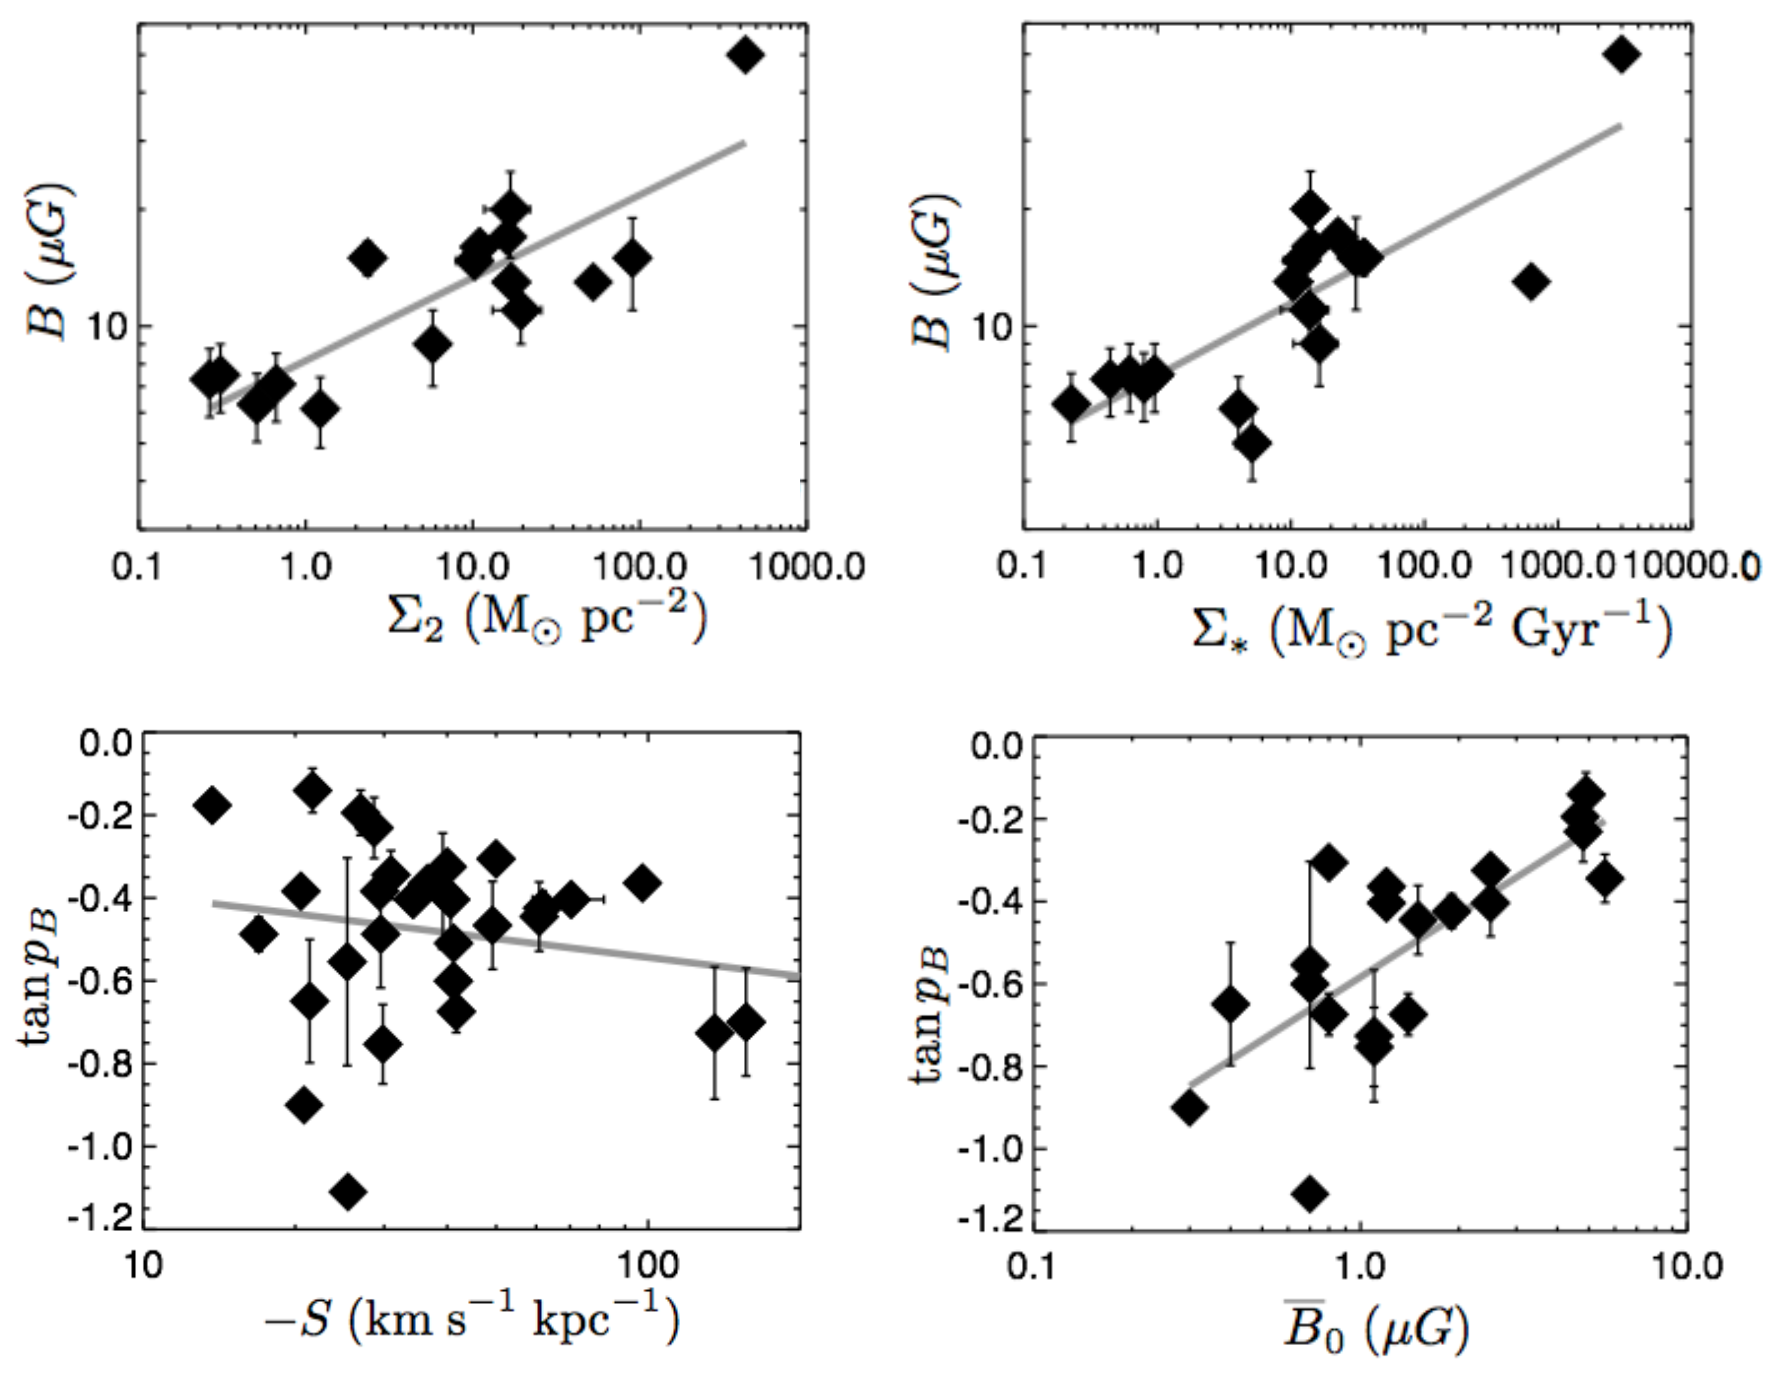
\includegraphics[width=0.48\textwidth]{VanEck.png}
%\end{center}
%\vspace{-6mm}
%\caption{\label{fig:bfield_spirals} 
%  Magnetic field properties from a sample of 20 nearby spiral galaxies
%from Van Eck et al. \cite[][panels taken from Figures 4 and 9]{2014arXiv1411.1386V}.  Top row: Total
%magnetic field strength vs. H$_2$ surface density (left) and vs. star
%formation rate surface density (right).  Bottom row: Pitch angle of
%mean magnetic field vs. rotational shear rate (left) and
%vs. axisymmetric component of the large-scale magnetic field (right).
%While \cite{2014arXiv1411.1386V} find close correlations between a
%variety of properties, not all are easily explicable via galactic dynamo
%theory.}
%\vspace{-3mm}
%\end{wrapfigure}
Measurements of magnetic field properties in other types of local
galaxies have been made as well.  Field strengths in local elliptical
galaxies are believed to be on the order of $5-10$~$\mu$G, comparable to local
spirals, although with much smaller coherence lengths -- far smaller
than the size of the galaxy itself
\cite{1993A&ARv...4..449W,1996MNRAS.279..229M}, though to date no conclusive
measurement has been made.  Field strengths in
dwarf galaxies have been measured to have total 
strengths ranging from $5-15$~$\mu$G and ordered fields having strengths
of $1-8$~$\mu$G, generally a few times weaker than local spirals,
depending on the galaxy in question
\cite{2000A&A...355..128C,2011A&A...529A..94C,2012MNRAS.423L.127R,Mao12,2013MNRAS.435..149N,2014A&A...567A.134J}.
We do note that dwarf galaxies with lower masses do tend to have lower
total and ordered magnetic field strengths than larger dwarfs
and spirals, and galaxies with higher star formation rates also
tend to have higher magnetic field strengths (as was seen in spirals
in \cite{2014arXiv1411.1386V}).  Furthermore, it seems that, for dwarf
galaxies where the structure of the magnetic field strength can be
measured, the ordered component is about $20\%$ as strong as the total
magnetic field, which is comparable to much more massive local spiral galaxies.

\vspace{-3mm}
\subsection{The Milky Way}
\label{sec:milkyway}
\vspace{-2mm}

The best candidate for obfuscating the picture of magnetic fields in galaxies is
our own Milky Way.  The proximity to the source means that high resolution
measurements can be made, but our location within the galactic disk means that comparing
to other galaxies is difficult.  Faraday rotation and polarization of other
galaxies measures the field strength integrated through the entire thickness of
the disk, while similar measurements of our own galaxy only sample fractions of
the field.  Further, many local radio features (such as the north
polar spur and other magnetized loops and filaments) make it difficult
to disentangle larger-scale magnetic field structures.

The magnetic field in the Milky Way's disk can be broken into two
components: a large scale magnetic field that has a coherence length
on the order of the size of the Galaxy itself, and a small scale field
that is either completely random or somewhat correlated with the large
scale field.  Synchrotron radio emission indicates that the large
scale field strength is roughly 10 $\mu$G at a Galactocentric radius
of 3 kpc, and decreases to 6 $\mu$G near the Sun.  This is consistent
with Zeeman measurements of nearby molecular clouds (see Section
\ref{sec:conngalmcs}).  Estimates of the strength of the random
magnetic field component varies from $B_{\rm{rand}} \gtrsim
1.3$~$\mu\rm{G}$ \citep{Gaensler01} to $4$~$\mu\rm{G}$
\citep{Fauvet11}.
The most complete survey of dust polarization was performed by the
\emph{Planck} satellite \citep{PlanckIntermediateXIX15}, which can be seen in
the right panel of Figure \ref{fig:bfield_morphology}.  Clearly structure can
be seen on a range of scales throughout the galactic disk.

The morphology of the magnetic field in external spirals is generally parallel
to spiral arms, as shown in the left panel of Figure \ref{fig:bfield_morphology}.  This is
likely the case with the Milky Way.  However, unlike other galaxies, the Milky Way
seems to additionally harbor at least one reversal in the direction of the
magnetic field
\citep{Thomson80, Jaffe11}.  Many models exist to match the data \citep[see the
recent review by][]{2015ASSL..407..483H}, including an antisymmetric spiral (similar to
other galaxies), a bisymmetric spiral (which would account for reversals), a
ring structure, and some superposition of these.  The vertical component of the
Galactic magnetic field is similarly difficult to measure.  Using rotation
measure from more than 1,000 extragalactic radio sources, \cite{Mao10} find
that there is no symmetry in the vertical component at the radius of the sun,
with the Galactic north field showing a field consistent with zero, and the
Galactic south field of $0.31 \pm 0.03 \mu$G.  On the other hand,
\cite{Jansson12} find that, modeling the synchrotron intensity from WMAP, the
field is consistent with an ``X'' shaped magnetic field.
Unfortunately, none of the existing measurements are 
consistent with expected observations and a coherent dynamo. This is
possibly due to the fact that the timescale for the coherent $\alpha-\Omega$
dynamo is longer than the age of the Galaxy, or if tidal interactions or
injection of small scale magnetic fields continually disrupt the symmetry
\citep{Moss12}.  

Another potentially important reservoir of  magnetic field energy is in the Milky Way's
circumgalactic medium (CGM), which is the huge volume of hot, diffuse
baryons that exists outside of the stellar disk but within the virial
radius of the dark matter halo.  The CGM  contains approximately half
of the baryons in the entire Milky Way system \citep[see,
e.g.,][]{2014ApJ...786...54P}, and is considered to be important for
the regulation of the star formation history of galaxies, and also responsible for
controlling the bulk scaling relations  seen in local galaxies
\citep{2015ApJ...808L..30V,2017ApJ...845...80V}.  The CGM is
metal-enriched, and thus is likely to be
substantially magnetized assuming that both metals and magnetic fields
originate in stars.  Some evidence exists for large-scale
magnetic fields in the CGM \citep[see,
e.g., Figure 7 in][]{2017ARA&A..55..111H}, but the detailed structure
of the circumgalactic magnetic will require the Square Kilometer Array
or one of its pathfinders as a probe \citep{2015aska.confE..41H}.

\red{GET REFERENCES}
One of the primary motivations for this study is the spatial distribution and
correlations in the magnetic field, and the synchrotron and polarized dust
emission that is dictated by these correlations.  These signals occupy different
locations in the galaxy, with the polarized dust emission at relatively low
galactic scale height and the synchrotron coming from higher, hotter gas.  Both
of these signals are foregrounds for studies of the polarized cosmic microwave
background, and will need to be properly understood if they are to be removed
from the signal.  The relevant quantities to study are $E$ and $B$, which are
rotationally invariant quantities related to the polarization intensity and
direction, and their spectral amplitudes, $C_\ell^{EE}$ and $C_\ell^{BB}$.  It has been found 
that these amplitudes scale as a powerlaw in the wavenumber, $\ell^\alpha$ where
$\alpha=-2.43$, and the is roughly twice the power in $E$ than $B$.  This is
intriguingly smooth over the high-latitude sky.  Preliminary studies \red{KIM}
\red{AK} have shown promising results.  \red{the bit about the location of the
synchrotron}

\begin{figure}[t]
\begin{center}
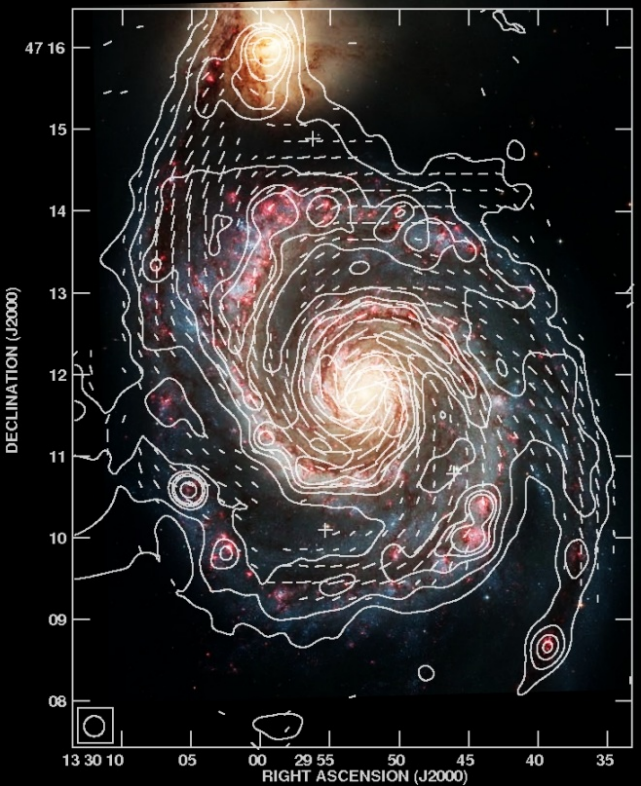
\includegraphics[width=0.29\textwidth]{Fletcher.png}
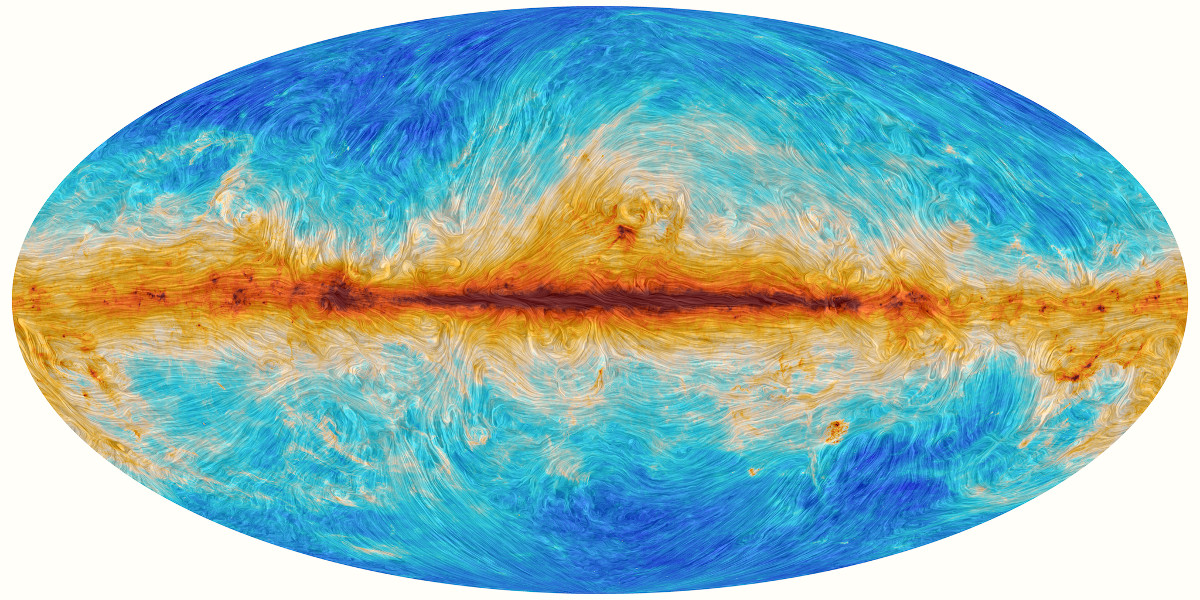
\includegraphics[width=0.69\textwidth]{Planck.jpg}
\end{center}
\vspace{-6mm}
\caption{\label{fig:bfield_morphology} Coherent magnetic structure is seen in
many disk galaxies. (\emph{Left}) The magnetic field from
polarized $\lambda=3,6$ and 20 cm  radio emission (vectors) along with total
emission (contours) in M51. From  \cite{Fletcher11}.  Optical background from \emph{Hubble Space Telescope}
(image credit: NASA, ESA, S. Beckwith (STScI) and The Hubble Heritage Team
(STScI/AURA)).  This shows the well-ordered nature of the magnetic field along
the spiral arms. 
(\emph{Right}) The \emph{Planck} polarization map showing the 353 GHz dust
intensity convolved with the direction of polarization
\citep{PlanckIntermediateXIX15}.  This shows coherent structrue on a range of
scales throughtout the Milky Way.
%(\emph{Right})  From \cite{Noutsos12}, the inferred magnetic
%field direction in the Galaxy (green vectors) as compared to spiral arms (white
%boxes).  Measurements from rotation measure from 622 pulsars, with field
%direction towards the sun in blue, red away from the sun.  Clearly reversals in
%the mean field are seen in the Galaxy, but not in M51
}
\vspace{-3mm}
\end{figure}

\vspace{-2mm}
\subsection{Connecting galaxies to molecular clouds}
\label{sec:conngalmcs}
\vspace{-2mm}

%This impacts our
%understanding of cloud formation as well as cloud lifetime and collapse, and,
%ultimately, star formation rates, masses, and binary rates.  Clearly there is
%order on the tens of kpc scale (e.g. Figure \ref{fig:bfield_morphology} from
%\citet{Fletcher11}), which is much larger than the 1-100 pc scale of molecular
%clouds.   
%The galactic magnetic field also has small-scale fluctuations
%\citep{2015ASSL..407..483H}, which is unsurprising as the ISM is also clearly 
%turbulent.  Simulations of multiphase magnetized ISM result in molecular gas with
%weak magnetic fields \citep{deAvillez05, Kritsuk09c}, while observations are
%ambiguous, 


Molecular Clouds and Giant Molecular Clouds are cold (10 K) and have masses
anywhere from $10^4-10^7$~M$_\odot$.  From the limited number of Zeeman splitting measurements in cold molecular
clouds, field strengths in molecular clouds range from 1 $\mu$G in low
density  gas ($\simeq 100$ \percc), and increase to a few mG in higher density gas
($\simeq 10^7$ \percc) \citep{Crutcher12}.  Star formation is controlled by some
combination of gravity, turbulence, and magnetic fields \citep{McKee07}, and 
the relative
importance of each is the subject of significant debate \citep[compare, e.g.,][]{Padoan13,
Li14}.   
The ratio of
magnetic to kinetic energy is typically parameterized by the \alf\ Mach number,
$\alfmach=v/v_{\rm{A}}$, where $v_{\rm{A}} = B/4 \pi \sqrt{\rho}$ is the signal
speed along a magnetic field line.  Values of $\alfmach>1$, so-called \sa\
flow, indicates a weak magnetic field relative to kinetic energy, while
$\alfmach<1$, or \suba\ flow, indicates that magnetic fields dominate energetically.  The ratio of
gravitational to magnetic energy is typically parameterized by the mass-to-flux
ratio, $\mu=M/\Phi$, where $\Phi$ is the magnetic flux threading a cloud of mass
$M$, in units of the critical field strength for collapse.  The actual values of
$\alfmach$ and $\mu$ are difficult to
measure observationally due to the challenge in measuring magnetic
field strengths directly over large scales
\citep{Crutcher12}. 
 Thus, statistical and morphological arguments are made,
often with different results.   From measurements of column density power
spectra and extinction measure distribution in molecular clouds,
\cite{Padoan99} and \cite{Padoan04c} argue that \sa\ turbulence is more
consistent with molecular cloud measurements than the statistics of \suba\
models.  On the other hand, \cite{Heyer12} have shown that a difference in the
slope of the velocity power spectrum between two orthogonal directions indicates that
$\alfmach\approx 1$.  Simulations \citep{deAvillez05, Kritsuk11c}
 indicate that
$\alfmach>1$ for clouds that formed from the warm neutral medium. 
Polarization
measurements indicate that fields are parallel to the long axis of low mass
filaments, 
perpendicular to the long axis of high mass filaments \citep{Li13}, and exhibit coherent
alignment between large and small scales \citep{Li09}, all of which indicate
$\alfmach<1$.
Zeeman measurements of methanol masers in star forming
region indicate that the
magnetic field order is imprinted on even small-scale structures over kpc
scales.
\citep{Green12}.  
However,
 turbulence substantially impacts the
structure of molecular clouds \citep[see, e.g.,][]{Elmegreen04, MacLow04}, and statistical
properties indicate that turbulent kinetic energy is comparable to, if not dominant over,
magnetic energy \citep{Padoan04, Heyer12}, indicating $\alfmach\gtrsim 1$.
Figure \ref{fig:SFR} shows the connection between molecular clouds and magnetic
fields, in the left panel, in observations of field alignment with spiral
structure, from \citet{2011Natur.479..499L}, and the connection between field
and the halo in a pilot study for the proposed work.

 The details of the initial conditions, boundary conditions, and
equation of state have profound impact on molecular cloud lifetimes and collapse rates
\citep{Federrath12, Collins12, Rey-Raposo14}.
Furthermore, even in
models of star-forming clouds where magnetic fields play a subordinate role their
effect is still non-negligible.  
Thus it is clear that for a
detailed understanding of star formation, magnetic fields must be included.
In order to capture these conditions self-consistently, \textbf{we will
perform extremely high resolution simulations of
isolated galaxies, extracted from cosmological initial conditions, that resolve the formation of a wide mass range of
molecular clouds.} 

%\dcc I cut this text.
%Magnetic fields can aid in the
%formation of molecular clouds by way of magnetic instabilities such as the
%Parker instability \citep{Parker66}, wherein buoyant, magnetized clouds of gas
%lose mass preferentially along magnetic fields into magnetic valleys, possibly
%%coalescing gas into massive structures \citep{Kim03}.  Alternatively, magnetic
%fields lend support against self-gravitating disk instabilities \citep{Kim01}
%and Jeans instabilities \citep{Elmegreen87}. 



\begin{figure}[t]
\begin{center}
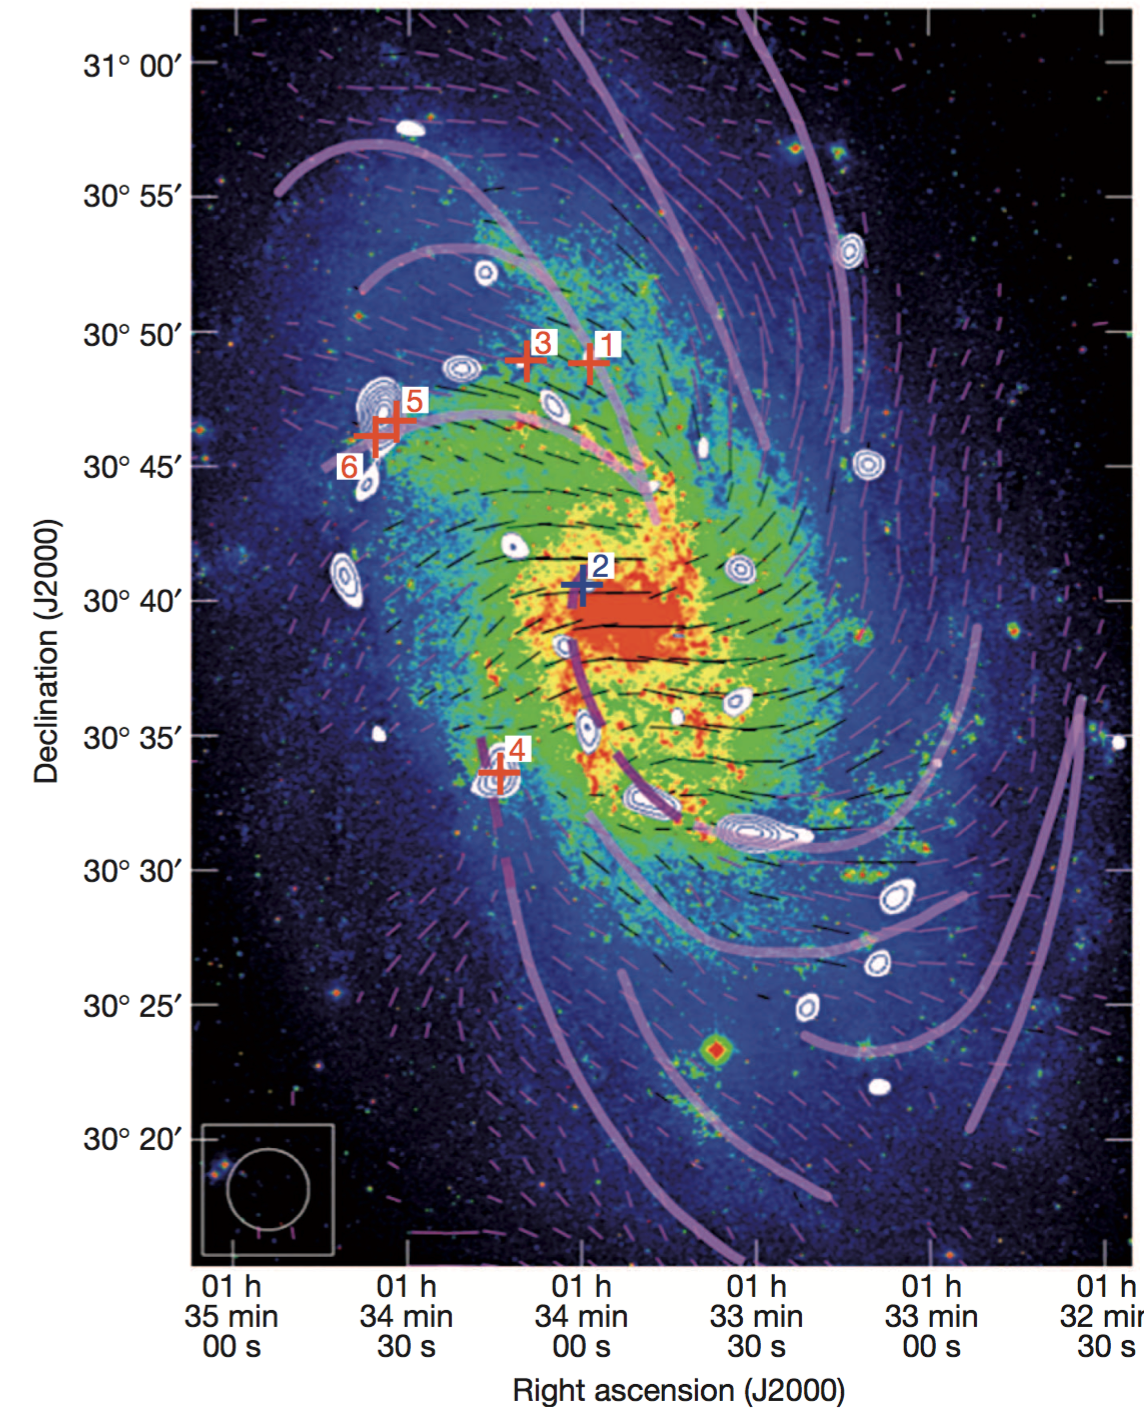
\includegraphics[width=0.23\textwidth]{LiHenning.png}
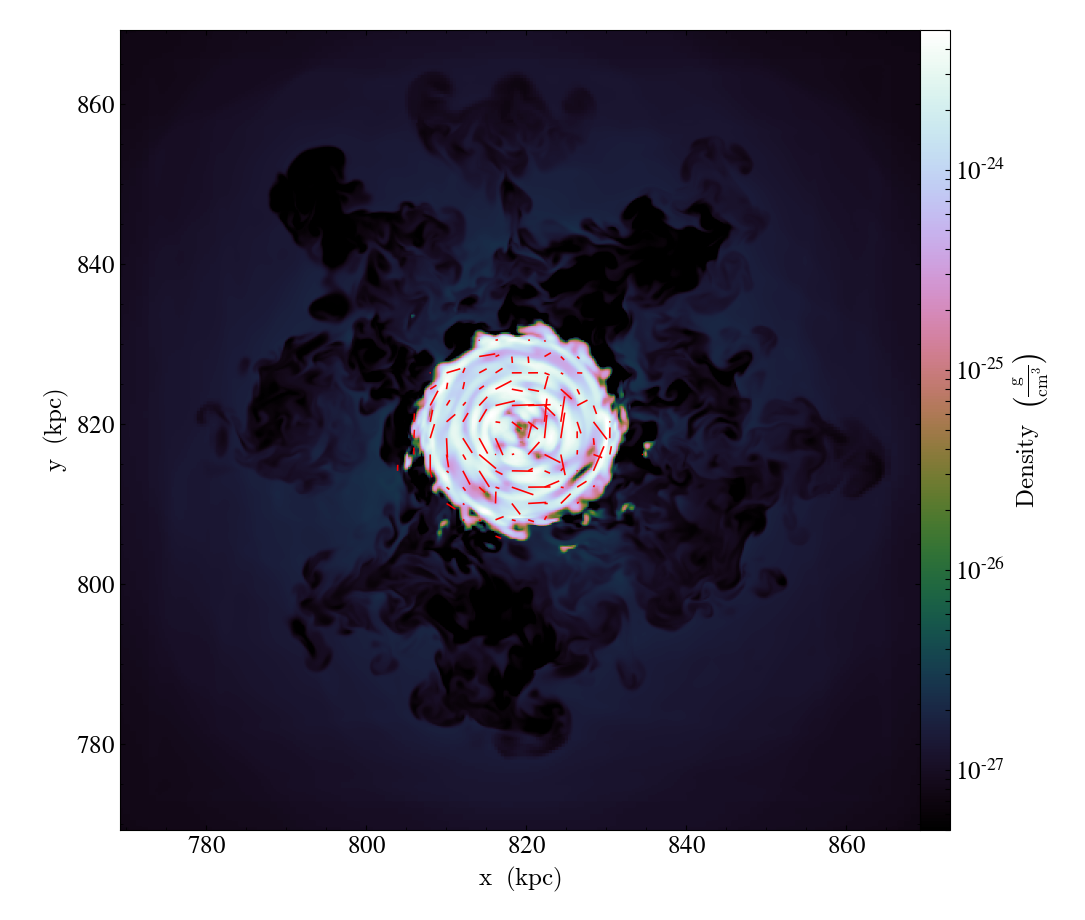
\includegraphics[width=0.346\textwidth]{g30_g18d_annotate_7.png}
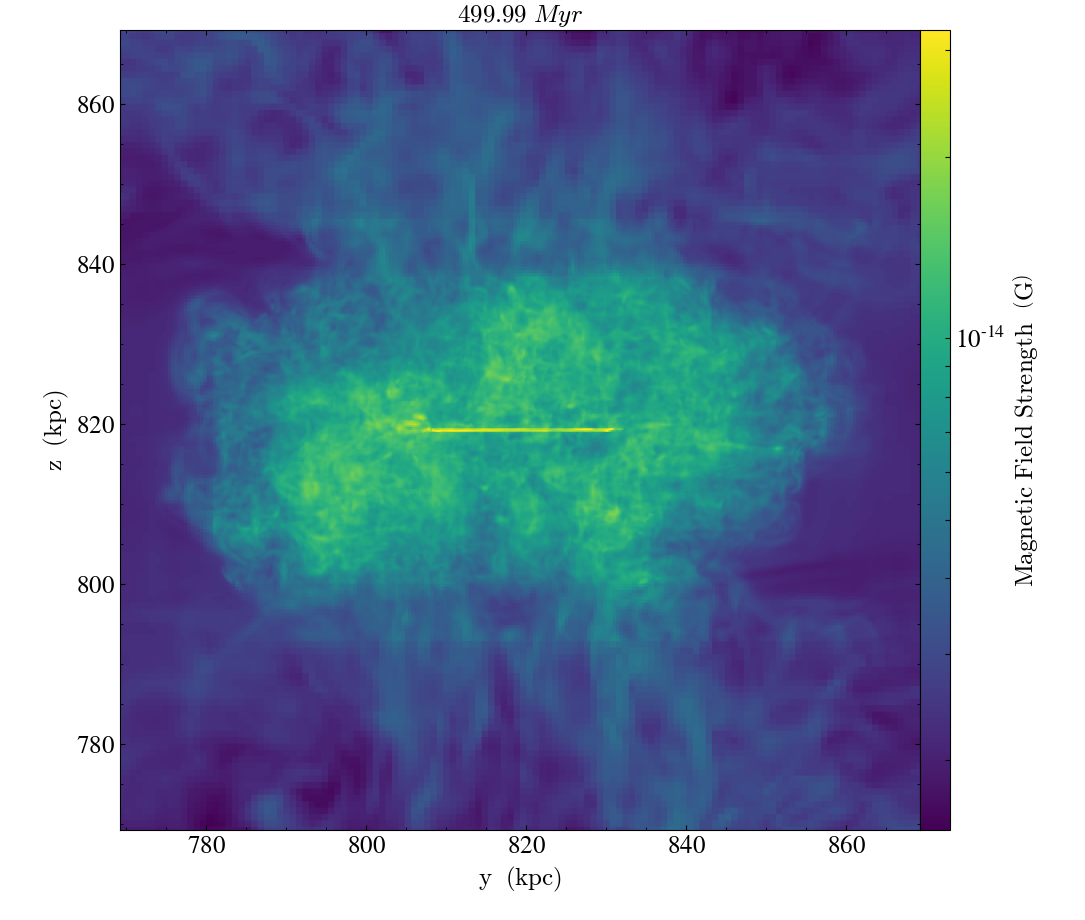
\includegraphics[width=0.346\textwidth]{g18d_0100_Projection_x_magnetic_field_strength_ones.png}
\end{center}
\vspace{-6mm}
\caption{\label{fig:SFR}
\emph{(Left)}: From \citet{2011Natur.479..499L}, magnetic fields in molecular
gas (thin lines) traces spiral arms (thick lines) in M33.
\emph{(Center, Right)} 
From preliminary galaxy-scale simulations with an initial
uniform field of $10^{-15}\rm{G}$ a Milky Way sized galaxy 
produces fields up to $10^{-13}\rm{G}$ at 20 kpc from the disk within 500 Myr.  
The center panel shows synthetic polarization direction following the rotational
structure.  The right panel shows mean magnetic field strength in an edge-on
projection.
This simulation has an
under-resolved ISM in the galaxy, and serves as a pilot study for the proposed
work. }
\vspace{-3mm}
\end{figure}

\vspace{-3mm}
\subsection{The origin and amplification of magnetic fields in the universe}
\label{sec:origins}
\vspace{-2mm}

% \brian Where do magnetic fields come from in the Universe?  Not 100\%
% clear yet.  High-z magnetogenesis; Biermann battery during structure
% formation and in stars; outflows.  In galaxies, mostly from
% stars/supernovae and amplification of existing b-fields due to the
% dynamo process.  Sum up MHD simulations of cosmological structure
% formation!

As discussed in Section~\ref{sec:extragalactic}, magnetic fields
appear to exist everywhere in the intergalactic medium, albeit at a
very low level.  The physical regimes where they appear to reside --
on megaparsec scales and above, and in both intergalactic filaments
and in voids -- argue against a galactic origin.  So, then, what is
the likely origin of these fields, and what theoretical constraints
can we utilize?

Widrow \cite{2002RvMP...74..775W,2012SSRv..166...37W} provides a host
of possible origins for the observed cosmological magnetic fields,
which we briefly summarize.  Magnetic fields could be generated during
the inflationary epoch, during the hadronic or electroweak phase
transitions, or in the radiation-dominated era prior to recombination.
Depending on the nature of the effect, theoretical predictions for a
minimum field strength vary hugely, from a minimum value of B~$\sim
10^{-32}$~G to substantially more than a Gauss (values given at the
present day).  Generally speaking, theory dictates that a minimum
magnetic field strength of $10^{-19}$~G (present-day value) and with
coherence lengths on megaparsec scales must exist; the maximum
theoretically-predicted value is vastly higher than the observational
upper limits from the CMB of $\bar{B} \simeq 10^{-9}$~G (Section~\ref{sec:extragalactic}).

Given the minuscule magnetic field strengths that must have been
generated prior to structure formation, and the relatively high ($>
10$~$\mu$G) fields observed in both galaxies and the cores of galaxy
clusters, an obvious question arises: how are such high magnetic
fields generated from such weak seed fields?  Straightforward
adiabatic collapse of the gas (and corresponding compression of the
fields) suggests an increase in magnetic field from the initial value
of $\delta^{2/3}$, where $\delta$ is the ratio of maximum to original
density.  Given the characteristic density of the Milky Way's
interstellar medium, this implies an adiabatic amplification of
$\simeq 10^4 - 10^5$ times the primordial value -- far too small of a
value to explain the roughly 13 order of magnitude difference between
the minimum inferred value in the lowest-density regions of the
universe and the field strength observed in the interstellar medium.

This observation leads inexorably to the conclusion that there must be
some sort of dynamo process at work that amplifies the magnetic field
by using kinetic energy from the various processes associated with
structure formation (i.e., gravitational collapse, rotational motion,
etc.).  There are two dominant modes of amplification.  The
\emph{fluctuating} dynamo draws small scale turbulent energy into
small scale magnetic energy.  While this mechanism has growth times of
$10^7$ years (fast enough to generate substantial fields from
extremely weak seed fields), it does not produce fields that are
ordered on large scales.  The second amplification mechanism is the
$\alpha-\Omega$ dynamo, wherein differential rotation and buoyancy
work together to add helicity to the fluid, thus amplifying the field
on the large scales associated with the rotation of the galaxy.  This
is a slower process, which limits the large scale field available to
more massive galaxies.  (See \cite{Brandenburg05} for a detailed
review of both dynamo processes.)  Either of these processes can
easily magnify a seed field to the galactic field
strength of $10^{-6}$~G \cite{Beck13}, and compression by
gravitational collapse further amplifies the galactic field strength
and is responsible for the further magnification of the field to the
$10^{-3}$~G level observed in high-density star forming regions
\cite{Collins11}.  We note that further seeds beyond the weak
primordial field may be necessary to reach the observed magnetic field
strengths in galaxies, particularly for the earliest galaxies --
observations of strong magnetic fields at high redshift imply that
dynamos have a relatively short time to operate!  If that is the case,
two plausible mechanisms for initial magnetic field generation are supernova
remnants \cite{2002RvMP...74..775W} and the jets from supermassive
black holes \cite{1969Natur.223..936H, 1990ApJ...364..451D}, both of
which produce strong magnetic fields with substantial coherence
lengths.



% Section 3: proposed work
\vspace{-4mm}
\section{Proposed Work}
\vspace{-3mm}


In this project, we will use high dynamic range magnetohydrodynamical
(MHD) simulations to understand how galactic-scale magnetic fields
affect the formation and evolution of molecular clouds, and to
identify the characteristics of these magnetized clouds that pertain
to star formation.  Specifically, we will use a targeted series of
high resolution MHD simulations of galaxy formation, both in a
cosmological context (Section~\ref{sec:cosmo_sims}) and as isolated, idealized
galaxies (Section~\ref{sec:molcloud_sims}), to explore the evolution
of magnetic fields through cosmic time.  

Each series of simulations will use
three main magnetic evolution assumptions: \emph{dynamo-only}  simulations,
wherein a weak seed field fills space at the beginning of the simulation, and
two \emph{feedback} recipes that vary the amount of field injected through
supernovae.  These \emph{feedback} recipes will use the toroidal injection
implemented in \enzo\ by \citet{Butsky17}.  This model deposits a fraction,
$\sigma$, of supernova energy in a toroidal configuration on the grid.  Our
large-field run will clone \citep{Butsky17} and use
 $10^{43}$erg per $\msun$ of initial
stellar mass, and our low-field run will use $1\%$ of that value.  For each of
the observational diagnostics,
(Section~\ref{sec:observational_comps}) we will perform synthetic observations,
matching noise and telescope resolution of the respective instruments, and
perform Baysian estimation to compare the four populations.  We expect that the
\emph{dynamo-only} simulations will fall short, which will allow us to bracket
the viability of our simulations.  In addition, we will perform the analysis on
the unfiltered simulations in the ``perfect telescope'' limit, which will allow
us to examine the ability of future SKA or Next Generation VLA observations to
explore these regions.

These calculations will be run with the \enzo\ and \enzoe\ codes
(Section~\ref{sec:codes}) using computing time secured through the XSEDE and
PRAC allocation processes (Section~\ref{sec:comptime_sims}).  \enzoe\ is the
developmental exascale successor to \enzo, and will allow us to perform much
larger simulations than \enzo.  The majority of the production simulations in
the proposed work will be suitable for either code.  



% From the cosmological simulation 
% These simulations will be used as initial and boundary conditions 

% \red{This will feed back to cosmological simulations as improved star
% formationa nd feedback algorithms, etc.}

% \red{need to elaborate upon this a bit before we dive into the
%   simulation section: we'll do simulations (described in 3.1), compare
% to specific observations (3.2), and will do this in a way that is
% logically partitioned (3.3).}


% Section 3.1 simulations
\subsection{Simulating the Magnetized Universe}
\label{sec:simulations}
\vspace{-1mm}

\subsubsection{Cosmological simulations}
\label{sec:cosmo_sims}
\vspace{-2mm}

As described in Section~\ref{sec:motivation}, there is a great deal of
observational evidence that magnetic fields exist in galaxies over a
wide variety of masses and redshifts, and also in intergalactic space.
Furthermore, it appears that the magnetic fields in star-forming
galaxies build up relatively quickly, based on observations of $z
\simeq 2-3$ galaxies which show that the magnetic fields measured in
their interstellar medium (ISM) are roughly in equipartition with
other sources of ISM energy.  We will explore the evolution of
magnetic fields in the universe, both over time and in a wide range of
environments, by using a carefully-chosen series of cosmological
simulations.  At present, a collaboration of galaxy modelers
(led by PI O'Shea) is in the midst of running two sets of
large-volume cosmological simulations using the \enzo\ code -- one of
a 25 Mpc volume, and the other 75 Mpc, both with $1024^3$ root grid
cells and particles, and with multiple sets of physics in each set of
calculations and moderate physical resolution ($\Delta \mathrm{x} \simeq 400$~pc).  Taken together, these sets of calculations resolve the
formation of galaxies over three orders of magnitude in mass, from
$\simeq 10^{10}$ to $10^{13}$~M$_\odot$, which encompasses galaxies
ranging in size from the Small Magellenic Cloud through the largest
ellipticals.  These simulations will be completed by the time that the
grant period for this project begins, and we will mine these datasets
to find approximately a dozen galaxies whose masses, morphologies, and
formation histories probe the regimes of interest for understanding
magnetic field behavior, and which we will resimulate at high resolution.  We will include
the following galaxies in our list of follow-up simulations,
which will enable us to target essentially the entire range of
observations listed in Sections~\ref{sec:extragalactic}
and~\ref{sec:lowz}:

\begin{enumerate}

\item Four spiral galaxies of roughly Milky Way mass (M$_{gal} \simeq 1-2 \times
10^{12}$~M$_\odot$) that have a range of formation histories,
including galaxies that have rapid early merger rates as well as those
with smoother formation histories.  In particular, we will include at least one galaxy
with a history similar to the Milky Way, with no major
mergers after $z \sim 2$.  These will be compared to observations of
local spiral galaxies \cite[e.g.,][]{2014arXiv1411.1386V} and to the
magnetic fields in the ISM of our own Milky Way.

\item At least two galaxies that grow rapidly at early times and are
large enough in terms of stellar mass that they can be directly compared to observations of magnetic fields
in L$_*$ galaxies at $z \simeq 2-3$
\cite[e.g.,][]{2008Natur.454..302B,2008ApJ...676...70K,1998A&A...329..809A}.

\item Four dwarf galaxies of masses $\simeq 10^{10}$ and $10^{11}$
M$_\odot$ at $z=0$, with one galaxy of each mass experiencing star formation
at the present epoch and one that is relatively quiescent.  These will be compared with
observations of local dwarf galaxies
\cite{2000A&A...355..128C,2011A&A...529A..94C,2012MNRAS.423L.127R,Mao12,2013MNRAS.435..149N,2014A&A...567A.134J}.

\item Two galaxies that are massive ellipticals (having essentially no
star formation) at $z=0$, which will be compared to local ellipticals
\cite{1993A&ARv...4..449W,1996MNRAS.279..229M}.

\end{enumerate}

Once these galaxies are selected from the pilot calculations, we will re-generate the initial
conditions for these galaxies at much higher mass and spatial
resolution using the MUSIC cosmological IC
code~\cite{2011MNRAS.415.2101H}, and then re-run the calculations to
the redshift of interest (typically the present day) at very high
spatial resolution ($\Delta \mathrm{x}_{min} \simeq 100$~pc) using
prescriptions for metal-dependent radiative cooling, star formation
and feedback, and AGN feedback.  This is the state of the art for
physics-rich cosmological galaxy formation simulations, and results in
galaxies with reasonable $z=0$ properties
\cite[e.g.,][]{2012MNRAS.423.1726S,2014MNRAS.444.1518V,2014MNRAS.445..581H}.
In addition, we will include the equations of ideal
magnetohydrodyamics using a cosmologically-motivated seed field
initialized to $B
\simeq 10^{-15}$~G at $z \simeq 100$ when the simulations begin.

One of the virtues of this type of cosmological simulation is that
they are relatively inexpensive (see Section~\ref{sec:comptime_sims}),
which allows us to experiment with variations in physical models to
understand the effect that model choice may have on our results.
Specifically, we will experiment with
the three magnetic field injection scenarios described the introduction to this
section.  

In addition to probing the questions posed in Sections
\ref{sec:objectives} and comparing to the observations described
\ref{sec:observational_comps}, we will
extract the galaxies at an appropriate point in their evolution and re-simulate,
as describe in Section \ref{sec:molcloud_sims}.  This will allow us to have the
most realistic initial and boundary conditions possible for the isolated
simulations.
%measure the strength and morphology of the evolved Milky-Way galaxies to
%ompare to those of the isolated galaxies, which will begin with idealized
%onditions () but, having substantially higher resolution, evolve in a more
%ealistic fashion.  

%As time and resources permit, we will 
%For some
%subset of these galaxies, in addition to our standard calculation we
%will try varying the strength and configuration of the initial seed field (which is unlikely to make a
%difference in larger halos~\cite[e.g.,][]{Xu10,Xu11}, though it is
%unclear if this is true in smaller halos), will experiment with
%magnetic field generation using the Biermann Battery
%\cite[e.g.,][]{Xu08,2014arXiv1408.4161G}, and explore multiple
%models for magnetic field injection from stellar populations and from
%AGN (in particular, varying the total energy and configuration of the
%magnetic fields injected).

%The cosmological simulations alone will allow us to answer several
%questions: How do magnetic fields develop in galaxies as a function of
%cosmic time, mass, formation history, and morphology?  Does the
%initial seed field's strength or configuration ultimately make a
%difference in the properties of observable magnetic fields in
%galaxies?  How are star formation rate and magnetic field properties related over
%cosmic time?
%And, finally, how (and to what distance) are magnetic
%fields communicated into the intergalactic medium, and can the
%inferred intergalactic magnetic fields
%\cite[e.g.,][]{1999ApJ...511...56K,2010Sci...328...73N} come from
%galaxies alone?  With this latter question, and assuming that most
%magnetic fields in the intergalactic medium come from galactic winds,
%we can potentially draw connections between metal absorbers in the
%intergalactic and circumgalactic medium with magnetic fields --
%connections that can be probed by the Jansky VLA, ALMA, and future
%long-wavelength telescopes such as the Square Kilometer Array.  Observational
%diagnostics will be discussed further in Section \ref{sec:observational_comps}


\vspace{-3mm}
\subsubsection{Galactic Simulations}
\label{sec:molcloud_sims}
\vspace{-2mm}

While the cosmological simulations will be able to directly address a
range of observationally-motivated questions about magnetic fields in
galaxies, their relatively limited ($\Delta \mathrm{x} \simeq 100$~pc) spatial  resolution means that they only
 marginally resolve larger molecular clouds, and are far too
coarsely resolved to directly simulate star formation.  To this end,
we will use our cosmological galaxy simulation data as initial
conditions for idealized calculations of isolated disk, elliptical, and
dwarf galaxies.  
For these calculations, we will extract the target galaxies from Section
\ref{sec:cosmo_sims} and embed them in isolated, non-cosmological boxes.  This will allow us to
increase the resolution to $\Delta \mathrm{x} \simeq 1$ pc and follow molecular cloud
formation, as well as more precisely model star formation and feedback
processes, albeit over substantially less than a Hubble time.
Fortunately, it has been observed that Milky-way sized galaxies have 
magnetic field strengths by $z\sim 0.5$ that are comparable to those
at the present day.  This indicates that the growth time
for such fields is quite short, so we will only need to simulate each galaxy for
a few $Gyr$.  

Recently, several groups have begun to explore magnetic fields in full-galaxy
simulations,  from cosmological initial conditions
\citep{Pakmor17}, in isolated, idealized
disks \citep{Rieder16, Rieder17, Butsky17}, and also focusing on large scale structure in
the IGM \citep{Vazza17}.  The proposed work will compliment these studies by
bridging the lengths scales and exploring the magnetic feedback.

With these simulations, we will
explore the relationship between large-scale galactic magnetization
and the properties of individual molecular clouds over a wider cloud
mass scale.
In addition, these
isolated calculations will allow us to explore in greater detail the
effects that varied energy and magnetic field injection mechanisms from stellar
populations (from stellar winds, AGB, and Type Ia and Type II
supernovae) 
have on magnetic field generation, and also on the possible
effect that resolution might have on dynamo amplification of magnetic
fields in both spiral and elliptical galaxies \cite[an effect that was shown to
be important in high-redshift halos;
][]{2010ApJ...721L.134S,2013AN....334..531S}.

In these simulations we will focus resolution on the cold molecular gas
and follow the injection of kinetic energy from supernovae, and the subsequent
dynamo. This will be done for one of each of the four categories of galaxies:
one spiral, one high-redshift galaxy, one dwarf, and one massive elliptical.  The
massive elliptical, having no star formation or molecular content, may be
omitted based on the magnetic activity seen in the cosmological phase. 
Each of these will be treated with three
magnetic feedback routines: the
plain \emph{dynamo-only} evolution, evolving with the field given by the
cosmological simulation; and the two toroidal feedback methods.  
Our work will attempt to incorporate the latest knowledge in simulating the
supernova driven ISM \citep[e.g.][]{Hill12, Shetty12b, Kim15b, Walch15, Padoan16} to the extent it is numerically feasible.  
The thermal
feedback from supernovae
and thermodynamics will target the formation of molecular clouds.  Supernovae
will be tied to star particles in order to be self-consistent, and inject
$10^{51}\rm{erg}$ of energy and a fraction of that in toroidal magnetic energy,
following \citep{Butsky17}, with the fraction depending on the simulation suite.
Thermal energy will be deposited in a sphere containing 60~\msun, following
\citep{Joung06, Hill12}, in order to keep the gas from radiatively cooling on
an unphysically short time scale.
Chemistry and thermodynamics will initially attempt to 
follow the description in the thorough study by \citep{Walch15}, which
simulated $\rm{H}^+, \rm{H}, \rm{H_2}, \rm{C^+}, \rm{CO}$.  This may provide
computationally prohibitive, in which case we will resort to heating and colling
based on tabular interpolation computed with Cloudy \citep{2014ApJS..211...19B, Ferland17}
and a density-based CO map.  
The chemistry is presently contained in the chemistry solver in \enzo\
\cite[see, e.g.,][]{Tasker11,2014ApJ...783...75M}.

The toroidal feedback has been implemented in \enzo\ using the hyperbolic
divergence scheme \citep{Dedner02}.  This will be extended to include the
Constrained Transport scheme \cite{Gardiner05, Collins10}, which conserves the divergence of the magnetic
field to higher precision.  This is theoretically straightforward, but
experience of the team has shown that ensuring field update stays consistent
across multiple refinement levels and in parallel has a number of technical
subtleties that make it unsuitable for an inexperienced graduate student.  In
order to ensure the code development aspect of this project is brief, we are
requesting a postdoc to carry out this work.  

%These simulations will allow us to refine the star formation and feedback
%algorithms by more finely resolving the sampled IMF and more finely resolving
%the turbulence and dynamo action. They will also allow us to explore the
%creation and destruction of molecular clouds in a magnetized environment, which
%has had little study to date \citep{Dobbs08, Kim15}, and the connection between the
%magnetic field of individual clouds to the galaxy itself.  The
%simulations described here will likely require a more detailed
%treatment of H$_2$ formation -- including dust grain formation,
%photoelectric heating, the effect of non-trivial optical depths on
%cooling rates, and others -- which are already contained in the \enzo\
%chemistry solver \cite[see, e.g.,][]{Tasker11,2014ApJ...783...75M}.
%In roughly half of the simulations we will inject magnetic fields from
%supernovae explosions, by adding it in a divergence-free manner as was done in
%\citet{Li06b, Nakamura06, Xu08c}, modeling the injection of magnetic energy into
%the ISM by supernovae.  This  will be compared to
%simulations that have no injection and only allow the small- and large-scale
%dynamos to operate, as in \citep{Beck12}.  



\davedeletenew{
\vspace{-3mm}
\subsubsection{Connecting Star Formation Theory and Galaxy Formation}
\label{sec:connections}
\vspace{-2mm}
}

%\vspace{2mm}
%\noindent\textbf{Connecting Star Formation Theory and Cosmology} 
%\vspace{2mm}

\davedeletenew{
\noindent Simulations of galaxy formation and star formation in a cosmological context
rely, by necessity, on ad-hoc prescriptions for star formation.  For instance,
the oft-used method of \citet{Cen93} requires that material is above a certain
threshold and has negative velocity divergence (i.e., converging gas
flow), then turns a fraction of gas in a resolution element
into stars.  This type of algorithm has a number of free parameters that are
typically normalized by their ability to reproduce observed star formation
properties of star forming galaxies.   Meanwhile, a substantial amount
of work has gone into understanding the rate and mass fraction of star formation
at the molecular cloud (MC) level.  In the proposed work, we will bridge the gap
between the local and cosmologial models by developing a new star formation algorithm that
incorporates developments in molecular cloud dynamics.  Ad-hoc star formation algorithms have done reasonably well  in
reproducing observable quantities such as the redshift evolution of stellar mass in galaxies.  However, the tight, linear
correlation between total gas mass and star formation rate, even at high
redshift, implies that the details of the giant molecular clouds are essential in determining star
formation rates \citep{Genzel10,Shapley11, Lada12, Lada14}.  \textbf{We will
develop a new star formation algorithm for use in cosmological simulations that
takes advantage of molecular cloud physics.}  This development will happen in
conjunction with both molecular cloud and cosmological simulations.
%%%paragraph
Predictions of the mass distribution and rate of star formation can be made
based on the statistics of the turbulence at the molecular cloud level.  We will
follow the pioneering work of \citep{Padoan02, Krumholz05} and the later
extensions by \citep{Hennebelle08c, Padoan11, Hennebelle11, Federrath12} to
formulate a new star formation procedure that incorporates the magnetic field of
the galaxy and molecular cloud properties.
%%%paragraph
One of the most fortuitous events in the study of supersonic turbulence is the
fact that the density probability distribution function (PDF) tends to form a
lognormal.  This has been exploited by several star formation models, and we
will do the same in this project.  The width of the PDF is related in turn to the Mach
number $\mach=v_{\rm{rms}}/c_{\rm{s}}$: higher \mach\ yields higher compression, thus
wider PDFs.  Using the standard turbulent and magnetic scaling laws, one can
formulate an analytic expression based solely on the mean Mach number, magnetic
field strength, and cloud mass.  Several variations of this have been
done, and we
will explore each in turn.  A similar model  was recently developed  with the
code Nyx \citep{Braun15}, wherein it was demonstrated that this technique is
successful in reproducing observed star formation laws.  We will extend this
work by additionally incorporating magnetic fields, in order to directly
incorporate MHD effects into our cosmological simulations
}


\davedelete{
Another fortuitous event is that the width of the
density can be related to the Mach number.
\begin{align}
p(\rho) d\ln \rho &= \frac{1}{\sqrt{2 \pi \sigma^2}} e^{-(\ln\rho -
\overline{\ln\rho})^2/(2 \sigma^2)} d \ln\rho \\
\sigma^2 &= \ln(1 + b^2 \mach^2),
\end{align}
where $\rho$ is the density of gas in units of the mean, $\overline{\ln\rho}$ is
the mean, $\sigma$ is the width of the PDF, and $b$ is a number of order unity.
Experimentally, $b$ ranges from 1/3 for incompressible flow to 1 for fully
compressible flow.  This PDF can in turn be used to predict a star formation
rate by noting that above some threshold, $\rhoc$, a parcel of gas will have a
Jeans mass smaller than the mass of the parcel, and will thus collapse to form
stars.  The effective Jeans mass should incorporate not only the gas pressure,
but also the magnetic pressure and turbulent pressure as well.  Several methods
to incorporate these additional forces will be include in our model,
and details
can be found in \citep{Krumholz05, Padoan11, Hennebelle11, Federrath12}.  
The final rate 
\begin{align}
\rm{SFR} &= \epsilon \int_{\rhoc}^\infty \rho V(\rho) d\rho \\
& = \epsilon \left (1+\rm{erf}\left[\frac{\sigma^2 - 2 \ln \rhoc}{3} \right]
\right),
\end{align}
where SFR is the star formation rate that will be used to determine the mass of
stars in zones.  
The work of \citet{Hennebelle11}  predicts the
initial mass function (IMF) 
from a fragmenting turbulent cloud based on an extension of the
Press-Schechter model to include a lognormal density fluctuation, rather than a
Gaussian, and is further extended to include a Jeans mass that depends on
turbulence and the magnetic field.  This model predicts the IMF from only the properties of the local gas.  
The
difference between this model and other ad-hoc star formation models is that
these parameters are drawn from the physical conditions in the cloud itself,
rather than an adjustable parameter that is set in order to reproduce the
Kennicut-Schmidt law.  
In 
our cosmological simulations, we will be restricted to a
fine-resolution grid of $\simeq 100$ pc,
which is larger than a typical star forming cloud.  Thus in order to model the
typical $\mach$ number and mean magnetic field strength  in our gas, which are
both necessary for the star formation recipe,  we must employ a subgrid scale
model (SGS).  Here we will use a combination of the AMR SGS model
\emph{Fearless}  \citep{Maier09}, which has been implemented in \enzo, and extend
it to include the effects of MHD based on the formulation outlined in
\citep{Chernyshov14}.  In this phase we will only worry about the subgrid
production terms, treating them as a passive quantity as far as the evolution of
the galaxy goes, and feeding them into our equation.
We 
will perform a suite of simulations examining the connection between star
formation on the molecular cloud level and the impact of magnetic fields.  A
significant distinction between the models for cutoff value is the treatment of
magnetic fields.  The work of \citet{Krumholz05} ignores them, while
\citet{Padoan11} treats the additional support of magnetic fields on equal
footing with the turbulence.  Simulations comparing these models will be
performed.
}

\vspace{-3mm}
\subsubsection{Computing time}
\label{sec:comptime_sims}
\vspace{-2mm}

Zoom-in cosmological simulations of a single Milky Way-type galaxy
using \enzo, with $\simeq 400$~pc resolution, require approximately
100,000 CPU-hours on TACC's Stampede resource
\cite{2012ApJ...749..140H,2012ApJ...759..137J,2013MNRAS.430.1548H}, or
slightly less on NCSA's Blue Waters.  The addition of MHD roughly
doubles the computational cost, and increasing the particle mass
resolution by a factor of 8 (to $5 \times 10^5$~M$_\odot$) will help
to resolve early structure formation, but will increase the
computational time by another factor of approximately four (rather
than 8, due to judicious choices made during the creation of initial
conditions that will reduce the overall number of particles).
Increasing spatial resolution will result in approximately a factor of
two increase in cost.  Together, this suggests that a high resolution,
physics-rich Milky Way-type simulation will cost roughly 100,000
node-hours on Stampede2 or Blue Waters -- expensive, but not impossibly
so.  Dwarf galaxy simulations and galaxies that stop at $z \simeq 2$
will require substantially less time.  Isolated disk simulations will
be comparably inexpensive -- at most 2,500 node-hours apiece on either
Stampede2 or Blue Waters.  Taken together, we estimate that we will
need 0.5-1 million node-hours per year on a machine like Stampede2 or
Blue Waters for the cosmological and isolated disk calculations
required for this proposal.

Dr. O'Shea and Dr. Collins have had significant success in procuring
computing time on XSEDE resources as PIs and Co-PIs of numerous large
allocation -- they have over 25 million combined core-hours of XSEDE
computing time over the past five years, most recently on XRAC
allocations TG-AST090040 and AST140008.  In addition, Dr. O'Shea was
the PI of a Blue Waters PRAC allocation that ended in March 2015
consisting of 124 million CPU-hours, and Drs. O'Shea and Collins are
co-PIs of a  Blue Waters allocation (continuing through March 2018) 
of roughly 100 million CPU-hours.    Both PIs will pursue additional
computer time on XSEDE resources and and Blue Waters (or its
progenitor system) that will be devoted primarily to the
project described in this proposal, and the level of resources
obtained is more than adequate for the proposed science.

% \subsubsection{Enzo-P -- maybe}

% \red{do this only if we have time and feel like making this a CDS\& E proposal!}


% Section 3.2 observational comparisons
\vspace{-3mm}
\subsection{Observational Comparisons}
\label{sec:observational_comps}
\vspace{-2mm}

We will perform synthetic observations of simulations using each of the
three magnetic feedback methods described in the previous section, and
will compare them
to a number of recent important observations.  Each comparison will use the
observed data from the literature, synthetic observations employing tools previously
developed by our team and previous collaborators
\citep[e.g.,][]{2013ApJ...765...21S,Barrow17,Barrow17_FL2}, convolved with
resolution and noise appropriate for the target measurement.  We will also
employ ``perfect telescope'' observations directly from the data.  Where
possible the data reduction tools of the particular telescope will be used \citep[e.g.,
CASA; ][]{McMullin07}.
This will allow us to do two things: first, we will verify the physical picture of
our simulations, allowing us to isolate problems or
success with the calculation; second, we will test our basic hypothesis, that
magnetic feedback from supernova explosions is an essential piece of the
magnetization of the universe.  Finally, we will make
predictions for measurements that will be made by both current and
future observatories.  These will primarily target next-generation radio
telescopes and their pathfinders, as well as JWST and WFIRST.

Our catalogue of observations will include the following: synchrotron emission
polarization; Faraday rotation measure and rotation measure synthesis; CO
emission, assuming a conversion from CO-to-H$_2$ appropriate for the system
\citet[e.g.][]{Genzel12,Clark15}; star
formation tracers such as H$\alpha$ and FIR luminosity; and Zeeman Splitting in
dense cores.

\vspace{-3mm}
\subsubsection{Extragalactic Observations}
\vspace{-2mm}

We will compare our simulations to Faraday rotation measures from
observations of high-redshift galaxies
\cite{2008Natur.454..302B,2008ApJ...676...70K,1998A&A...329..809A},
the field magnitude and arrangement in local dwarf galaxies,
\cite{2000A&A...355..128C,2011A&A...529A..94C,2012MNRAS.423L.127R,Mao12,2013MNRAS.435..149N,2014A&A...567A.134J},
field strength, structure and coherence in nearby elliptical
\cite{1993A&ARv...4..449W,1996MNRAS.279..229M} and spiral galaxies
\cite{2014arXiv1411.1386V}.  We will also use measurements of
large-scale intergalactic magnetic fields as a constraint
\cite{2010Sci...328...73N}.   
%RM measurements will include also include the
%use of depolarization of background sources to explore the field strength and
%turbulence of galxies
%\citep{Schulman92}.  
Recently techniques have been developed to combine polarized synchrotron
emission with Faraday Rotation depths to probe the full magnetic configuration
\citep{Heald09, Mao15}.
We will primarily aim to reproduce the morphology of observed integrated
polarization angles of galaxies \citep{Stil09}, the alignment of molecular
clouds and spiral arms \citep{2011Natur.479..499L}, and the relation between
field strength and galactic properties such as mass and velocity dispersion
\citep{2014arXiv1411.1386V,Tabatabaei16}.
We will then make predictions for (and thus
motivate) future observations of galactic magnetic field properties that will be
available to the current and future radio telescopes such as the Jansky VLA, ALMA, and LOFAR, and in the
further future the Square Kilometer Array pathfinder telescopes such
as ASKAP, APERTIF, MeerKAT, and
the SKA itself.

An extremely useful probe of the correlation of magnetic field properties and
star formation is the
correlation between the Far Infrared Radiation (FIR) flux and the
Radio Continuum (RC).  A surprisingly tight correlation between these
two fluxes has been studied for several decades \citep{Helou85}.  Both
radiation sources are indirectly related to star formation, and we
will aim to probe this correlation as a function of redshift.  The FIR
comes from re-heating of dust near sites of massive star formation,
while the RC comes form synchrotron radiation of cosmic rays
\citep{Helou93,Niklas97}.  \cite{Murphy06} model the radio profiles
as smoothed version of the FIR profiles, indicating that for the most
part the RC can be seen as a diffusive flux of cosmic rays.  However,
accurate measurement of this relation has not been reproduced in
cosmological simulations.  Modeling the FIR is done in post-production
after the simulations have finished, by measuring the mass
distribution in stars at a given time and using radiative transfer to
measure the optical depth to FIR.  Modeling the RC requires following
the cosmic ray spectrum and the competition between radiation terms.
These include inverse Compton scattering, ionization of neutral gas,
and bremsstrahlung in addition to the synchrotron that is observable in the RC.  \cite{Schleicher13b} propose that at high
redshift, inverse Compton may begin to dominate over synchrotron and the FIR-RC
correlation will break down around $z= 2-4$, depending on the strength
of the field and the star formation rate.  Several of our simulations
will include the cosmic ray treatment incorporated into Enzo and
described in \cite{Salem14,Salem14b}, suitably modified to incorporate
cosmic ray losses by the aforementioned processes.  This will allow us
to predict future observations by ALMA and LOFAR and to explore the
utility of the RC as a probe of highly extincted star formation.

Another important correlation is the ``Star Formation Main Sequence''
(SFMS) of galaxies \cite{Daddi07, Speagle14}. This relation
between star formation rate and stellar mass is a power law that is
essentially constant over time, with a normalization that falls with
time.  This can be interpreted as a relatively quiescent, steady-state
star formation process with cosmic time.  Recent simulation efforts
have reported good agreement with the SFMS at low redshift, but
reduced star formation rate at intermediate redshifts
\citep{Sparre15}.  We will measure this for not only the highly
resolved galaxies, but also the entire population of galaxies formed
from the cosmological simulation.  This will be compared to both the
low redshift behavior \cite{Brinchmann04} and the high redshift
properties \cite{Daddi07}.  This measurement itself is not a probe of magnetic
fields, but as star formation depends on field strength we will
correlate the slope and normalization of this linear relation with
magnetic field strength in the constituent galaxies.

\vspace{-3mm}
\subsubsection{Galactic Observations}
\vspace{-2mm}


One of the primary goals in this work is understanding the
relationship between the large scale magnetic field
of the galaxy and the magnetic fields in molecular clouds.  As discussed in Section \ref{sec:conngalmcs}, there is clear evidence of
coherent magnetic fields in galactic structure, but the importance in
molecular cloud structure and dynamics is ambiguous.  

The primary question is:
Over what scales are the magnetic field aligned, and how does this alignment
imprint on the molecular gas and impact its dynamics?  To properly answer this
question, we will focus on three measurements, ensuring consistency with earlier
observational work and exploring field properties that have not been measured.
These properties are: the properties of individual molecular clouds;
the correlation between field
directions at two points; and correlations between field direction and material
gradients.  

\noindent
{\bf Molecular Cloud Properties.}
The mean magnetic field strength in molecular clouds is challenging to measure,
but potentially of critical importance in star formation theory.  We will reconcile
molecular cloud properties with observational molecular clouds by comparing
synthetic $^{13}\rm{CO}$ maps with linewidth-size and mass-size relations as
measured by the Galactic Ring survey \citep{Jackson06,Roman-Duval10}.  We will
then predict the mean field strength vs. linewidth and size, and discuss the
expected mass-to-flux and kinetic-to-magnetic energy distributions.

\noindent
{\bf Field-Field Correlation.}
We will use 
synthetic polarization and Faraday rotation measure to measure the correlation
length in the galactic scale simulations.  We will also measure the distribution
of alignments of magnetic fields between and within individual molecular clouds,
and between each molecular cloud and the three-dimensional, kpc-scale
mean field.
These will be compared to the well-correlated alignment seen within molecular
clouds \citep{Li09} and  along galactic spiral arms \citep{Fletcher11}.  This will
allow us to ensure the validity of the fields in our galaxies, and predict the
probability of alignment between any pair of molecular clouds.

\noindent
{\bf Field-Mass Correlation.}
We will also explore the relation between field strength and material.  This has
garnered recent attention as magnetic field tends to align with low density HI
as seen in the GALFA-HI survey  \citep{Clark14}, and tends to lie perpendicular
to higher density structure \citep{PlanckXXXII14}.  We will perform synthetic dust
emission and synthetic HI maps to examine these properties.  Dust polarization
results will be compared to the histogram of relative orientation between
polarization angle and column density gradient. For consistent comparison with
the HI measurements, we will perform the Rolling Hough Transform \citep{Clark14} on the
synthetic HI map to determine the linear structure, and correlate that with the
polarization map.  These measurements will assess the validity of the data.  We
will also explore the alignment of clouds themselves on the large scale
patterns, and measure the probability of finding a cloud at a certain distance
along the large scale field.  This will measure the interaction of magnetic
field and structure on the 100-1000 pc scale.

\noindent
{\bf CMB Foregrounds}
We will also produce all-sky maps for the study of CMB foregrounds.  Maps of the
sky are necessary for training image processing and noise reduction algorithms,
an essential part of the success of future missions.  We will provide a suite of
all-sky maps for such purposes.  We will also measure the variation of
$C_\ell^{EE}$  and $C_\ell^{BB}$ with time and magnetic feedback prescription.
This will allow us to understand the constituent physics that sets $\alpha_{EE}$
and $\alpha_{BB}$.



%\red{CMB foreground stuff goes here}





% Section 3.3: the collaboration
%
\vspace{-3mm}
\subsection{Collaboration Structure}
\label{sec:collaboration}
\vspace{-2mm} 



% Section 4: Codes and methods (4.1 enzo, 4.2, yt)
\vspace{-4mm}
\section{Tools}
\label{sec:codes}
\vspace{-3mm}

% \brian  \dave  \red{maybe we want to get rid of this section, lose the yt
% discussion, and move our description of Enzo to section 3.1.3?  (I am
% a big fan of this)}
 
% \subsection{\enzo}
% \label{sec:enzo}
% \vspace{-1mm}

For this work, we will be using the adaptive mesh refinement (AMR) code \enzo,
and its exascale succcessor, \enzoe.
The former is a well-established code for many computational astrophysics
problems.  The latter is an AMR code that has been designed for extreme scalability on both CPU
and GPU architectures, but shares the same physics packages as \enzo.  The use
of both codes allows us to take advantage of the enormous performance gains of
\enzoe\ while still ensuring success of the project.  As \enzoe\ development is
completed it will supplant \enzo\ for our calculations.

\noindent
{\large \textbf{The \enzo\ code.}}
The calculations described in this proposal will be performed using
the \enzo\ code.  \enzo\ is a publicly available Cartesian adaptive
mesh 
refinement code used for the simulation of cosmological and
astrophysical phenomena

\enzo\
\cite[][\url{http://enzo-project.org}]{2014ApJS..211...19B}.  
uses a block-structured adaptive mesh refinement scheme 
\cite{Berger89} to achieve high spatial and temporal resolution, and
combines an N-body adaptive particle-mesh solver for dark matter
dynamics with a Piecewise Parabolic Method (PPM) hydro solver that has
been extensively 
modified for cosmological applications and hypersonic
flows \cite{Bryan95}.  In addition, the code includes a range of other
physics, including both equilibrium and nonequilibrium chemistry and
cooling models, radiative cooling using a Raymond-Smith model and
Cloudy emissivity tables \cite{2008MNRAS.385.1443S}, and prescriptions
for the formation and feedback of both stellar populations and black
holes.  \enzo\ also includes modules for magnetohydrodynamics (both
the Dedner divergence-cleaning method and a constrained transport
method; \cite{Wang:2009a,Wang:2010,Collins10}) and radiation transport
using a ray-casting method and flux-limited diffusion \cite{Wise11,
Reynolds09}.  \enzo\ has been used to model a wide variety of
cosmological and astrophysical phenomena -- most relevant to this
proposal, \enzo\ has been used heavily to study high- and
low-redshift cosmological structure formation \cite{Abel02, Turk09,
2007ApJ...654...66O, 2012MNRAS.427..311W, 2008MNRAS.385.1443S,
2012ApJ...749..140H, 2014ApJ...791...64E, 2013MNRAS.432.1989S}, the
intergalactic and circumgalactic medium
\cite{2007ApJ...671...27H,2011ApJ...731....6S,2013MNRAS.430.1548H,2012ApJ...759..137J},
and the properties of star-forming molecular clouds
\cite{Kritsuk11,Kritsuk11b,Collins11,Collins11b,Collins12,Schmidt13}.

%The \enzo\ code has been selected by the NSF to be part of the
%Petascale Computing Resource Allocation (PRAC) program under three
%separate allocations totaling approximately 300 million core-hours, and was one of
%the handful of codes that were first used on Blue Waters when it was
%first made available for science runs in early 2012.  Near-perfect
%scaling of the code in its unigrid (non-AMR) mode has  been
%demonstrated to more than 90,000 CPU cores.  Calculations using AMR do
%not scale as well, although reasonable performance at up to several
%thousand CPU cores can be expected for large, well-balanced, and
%physics-rich AMR runs.  Given that the simulations needed for this
%project are well below this scale, \enzo\ will easily handle the
%calculations that are necessary for the proposed work.

% \vspace{-3mm}
% \subsection{\yt}
% \label{sec:yt}
% \vspace{-1mm}

{\large \textbf{The \enzoe\ code.}}

\red{forest of oct trees.  salable gravity.  physics from enzo.  kokos.  cpu and
gpu.}

\enzoe\ \citep{Bordner12, Bordner18} is the Exascale successor to \enzo. 
It retains the physics solvers from \enzo\ (e.g. the PPM and MHD solvers,
chemistry, thermodynamics, star formation, etc) but replaces the AMR framework
with a highly scalable ``forest of oct-trees,'' which enables scaling AMR to
hundreds of thousands of cores. \citet{Bordner18} show \enzoe\ (branded Enzo-P
in that publication) scaling to 265,000 processors.  This kind of scaling is not
available to \enzo, but will be necessary for the future growth of computational
astrophysics.

\enzoe\ is currently under development under an NSF CSSI grant (\#OAC 1835426)  lead by the
collaborator, Dr. O'Shea.  At present the majority of physics solvers are
present and functioning in \enzoe.  The only outstanding piece of code
to be ported from \enzo\ to \enzoe\ is the \emph{flux correction} routines.
These routines ensure conservation across refinement jumps and are necessary for
accurately conserving mass and magnetic flux.  The PI and collaborator have ample experience with
these algorithms and foresee little difficulty in completing this development in
the first year.

\vspace{2mm}
\noindent
{\large \textbf{The \yt\ code.}}
Our simulations will be analyzed and visualized with the \yt\ package
\cite[][\url{http://yt-project.org}]{Turk11}, which is an open source
analysis and visualization toolkit for grid- and particle-based
simulations.  \yt\ was originally developed to work with \enzo, but
now supports numerous simulation codes, including both grid-based and
particle-based astrophysical codes (i.e., FLASH, ART, Gadget,
Gasoline).  Among the capabilities of \yt\ are slices and projections
(both on and off the Cartesian axes); volume renderings; halo finding
and profiling; 1, 2, and 3 dimensional profiles; light-cone
projections; synthetic QSO sight lines (i.e., absorption line spectra);
contouring; and clump-finding.  We will use \yt\ to perform many of
these analysis tasks -- all of which are parallelized -- and will
furthermore use \yt\ to make a variety of synthetic observations of
galaxies using tools that have been developed and used by our
collaboration \citep[e.g.,][]{Barrow17,Barrow17_FL2}.  \yt\ can be 
used as a standalone code and is also
callable from within an \enzo\ simulation, allowing analysis to be
performed on in-memory datasets (a capability that will be very
helpful for analysis of our larger simulations).  \yt\ is highly
parallel, scales well on XSEDE computing resources, and is currently
being optimized for the Stampede2 supercomputer.



% Section 5: significance of proposed work
\vspace{-4mm}
\section{Significance of Proposed Work}
\vspace{-3mm}

Magnetic fields are essential components of galactic structure, but
the nature of their growth and morphology is elusive to understand
from a theoretical and numerical standpoint.  The challenge in doing
so lies in the difficulty of devising a consistent treatment of
initial and boundary conditions, of including the necessary physics,
and in interpreting observations.  The proposed project will model the
origin and evolution of galactic magnetic fields, and their impact on
star-forming molecular clouds, from cosmological initial conditions to
the present day.  We will also create synthetic observations for JVLA,
ALMA, and other telescopes, which will be crucial to interpretating
existing and upcoming observations.  In addition, we will use these
tools to explore the possibilities of future observations that will be
made by the next generation of radio telescopes  (in particular, the ngVLA and SKA).  This work will
result in a deep understanding of the connection between galaxies and
molecular clouds, and of the magnetic fields that permeate these
objects.  This project is innovative due to its connection of
cosmological structure (i.e., galaxies and their environments) to
molecular clouds and the star formation that occurs therein, and the
modeling of both of these classes of objects in a unified theoretical
and numerical framework.  The understanding gained by doing this will
be transformative in terms of our ability to more accurately model
star formation through cosmic time, and will directly connect to
current and future observations of magnetic fields in a range of
astrophysical situations.


%\newpage

% Section 6: results from prior NSF support

%%%%%%%%%%%%%%%%%%%%%%%%%%%%%%%%%%%%%%%%%%%%%%%%%%%%%%%%%%%%%%%%%%%%%%%%%%%%
\vspace{-4mm}
\section{Results from prior NSF Support}
\vspace{-3mm}




%% \noindent \textbf{Dr. Brian W. O'Shea:} is currently the PI or co-PI
%% of multiple NSF-funded projects.  The grant most relevant to this
%% project is an NSF Division of Advanced Cyberinfrastructure Petascale
%% Computing Resource Allocation grant (PRAC; ACI 0832662; ``Formation of
%% the First Galaxies: predictions for the next generation of
%% observatories,'' PI: Brian O'Shea, \$40K, 5/2009-4/2013.
%% \textbf{Intellectual merit:} This grant examined high-redshift galaxy
%% formation using extremely sophisticated cosmological simulations that
%% included both radiation transport and detailed treatments of star
%% formation and feedback, and made detailed predictions about the
%% transition between metal-free and metal-enriched star formation as
%% well as the properties of populations of high redshift galaxies.
%% Publications from this grant include
%% \cite{2013ApJ...773...83X,2014ApJ...791..110X,2014ApJ...795..144C,2015MNRAS.452.2822S,
%% 2015ApJ...807L..12O, 2015ApJ...802....8A}, with additional papers
%% currently in the refereeing process.
%% \textbf{Broader Impacts:}  This project helped to improve the accuracy
%% of simulations of galaxy formation, which is crucial to making
%% predictions for a variety of ground- and space-based observational
%% campaigns.  It helped to train multiple graduate students and
%% postdoctoral researchers, and to make substantial infrastructure improvements  to the
%% \enzo\ and \yt\ codebases, which will benefit the user communities of
%% those tools.  Also, public talks relating to high redshift galaxies
%% and their importance to astronomy and astrophysics were given by
%% several of the investigators.


%\noindent \textbf{Dr. Brian W. O'Shea:} Dr. O'Shea has recently been
%the PI or co-PI of several NSF-funded projects.  The most relevant
%recent grant is an ongoing NSF Office of Advanced Cyberinfrsastructure
%Petascale Computing Resource Allocation grant (PRAC; ACI 1514580;
%``Petascale adaptive mesh simulations of Milky Way-type galaxies and
%their environments,'' \$31.5K, 8/1/2015-7/31/2018).  
%\textbf{Intellectual merits:} This
%project has created an extensive library of simulated
%Milky Way-like galaxies, their progenitors, and their environments,
%which can be used to explore a wide range of observable astrophysical
%phenomena.  The analysis of the simulations is ongoing, and are being
%used to interpret recent observations relating to the intergalactic
%and circumgalactic medium, galactic and extragalactic magnetic fields,
%and high redshift galaxy formation. The simulation data produced
%during the course of this project and resulting data products will be
%made publicly available, heavily leveraging this investment in
%computational resources.  \textbf{Broader impacts:} This project
%involves scientists in training at the undergraduate,
%graduate, and postdoctoral level.  Datasets have been visualized by
%the NCSA, and will be widely disseminated
%to the public.  Publications: \citep{Barrow17, Barrow17_FL2,
%2017ApJ...847...59H, 2016ApJ...833...84X, 2016ApJ...832L...5X}.
 
\textbf{Dr. David C. Collins:} Dr. Collins is PI on ``Magnetic Fields in the Formation of
Molecular Clouds, Filaments, and Cores'',  (NSF AST-1616026, \$298,492,
09/01/2016 - 08/31/2020)  which has been
examining collapse of pre-stellar cores and the role of magnetic fields therein.
We have focused on 1.) the initial conditions of pre-stellar core collapse 2.)
the energy budget of the collapse and rate-limiting processes and 3.) the work
done on the gas by magnetic forces.
\textbf{Intellectual merits:} This project is exploring the early phases of
pre-stellar cores with an aim to find the earliest precursors of star forming
objects.  \textbf{Broader impacts:} This project involves training graduate
students, and the data will be freely available upon the completion of the
project.  Publications are being prepared presently.

Dr. Collins was also Co-PI on 
an NSF Office of Advanced Cyberinfrsastructure
Petascale Computing Resource Allocation grant (PRAC; ACI 1514580;
``Petascale adaptive mesh simulations of Milky Way-type galaxies and
their environments,'' \$31.5K, 8/1/2015-7/31/2018)  \textbf{Intellectual
merits:} This project created an extensive library of simulated Milky Way-like
galaxies and their environments.  These will be used in the current proposal for
initial conditions of the cosmological simulations.  Publications: This has
resulted in the publication of \citet{Hummels19}.


% Section 7: management plan and timeline
%%%%%%%%%%%%%%%%%%%%%%%%%%%%%%%%%%%%%%%%%%%%%%%%%%%%%%%%%%%%%%%%%%%%%%%%%%%%
\vspace{-4mm}
\section{Management plan and timeline}
\label{sec:timeline}
\vspace{-3mm}

\textbf{The Team.}  

Dr. David Collins (Co-PI) is an expert in numerical MHD methods and
simulations of star forming clouds, and has participated in
simulations of MHD turbulence in a variety of contexts, including
first stars and galaxy clusters.  He was primarily responsible for
the development of the MHD solver that will be used for this work.  In
the proposed work, Dr. Collins will be responsible for directing the activity,
analysis of simulation products, and code development as necessary.


%University will be responsible for simulations at the galaxy scale and
%below, focusing on the formation and collapse of molecular clouds, and
%the strength and topology of the galactic magnetic field.  They will
%also be responsible for the development of the new MHD-based star
%formation and feedback algorithm, and will lead the design and
%analysis of idealized disk galaxy and ISM/molecular cloud simulations.

Dr. Brian O'Shea (external collaborator, Michigan State University) is an expert in cosmological simulations of
structure formation, and has modeled galaxy evolution from the
earliest galaxies through present-day galaxy clusters.  He is an
expert on the sub-grid modeling of astrophysical processes in the
\enzo\ code, and is wholly or partially responsible for several of
\enzo's most critical modules for this project, including the star
formation and feedback and AGN feedback algorithms.  In this work,
Dr. O'Shea and his research group at Michigan State University will be
responsible for the remaining \enzoe\ developments and interpretation of scientific results.

The proposal will also include one graduate student at FSU.  This student will
be responsible for performance of both cosmological and isolated galaxy
simulations and analysis of results.

\vspace{2mm}
\noindent
\textbf{Plan and Timeline.}

PI Collins will be responsible for
carrying out the research described in this proposal and for reporting
progress and results to the NSF, and will be responsible
for overseeing the grant budget and for mentoring the graduate student.

Dr. O'Shea and the team at MSU are responsible for the final development needs
of \enzoe, and will aid in the interpretation and analysis of results.

The proposal will provide support for one unnamed graduate student.  As the
student has not been selected, we will structure the timeline assuming an
inexperienced student.  

The timetable and milestones for this project are listed below.  We
assume for planning purposes that the work done as a part of this
project will start in August 2020.
This project runs the risk of being overly ambitious.  
New code development 
brings uncertainties, and there are more interesting questions to be asked of
the resulting simulations than we can possibly ask with the personnel involved.  Here we describe a minimal and conservative work
plan to ensure success of the primary measurements.  To hedge against code
errors and development setbacks, the initial phases will be run with both Enzo
and \enzoe.  This will result in some additional cost as the number of
simulations and their setup will increase, but the redundancy will ensure a
successful results while verifying results from the new code.  Once development
of \enzoe\ is finished, it will be used exclusively.  In the unlikely event
of severe delays, Enzo will be used for the production simulations. 

The basic sequence of simulations for our research plan is as follows:
\begin{enumerate}
    %\item Get the magnetic feedback working with CT (maybe ignore that)
    \item Perform a galaxy formation simulation at cosmological scales
    \item Extract galactic properties from a target galaxy
    \item Simulate isolated galaxy
    \item Produce synthetic observations
\end{enumerate}
Each of these actions uses machinery that has been well tested in \enzo\ and
\yt.  
Using \enzo\ and simple physics and low resolution (e.g. no MHD or supernovae
and small enough to fit on a desktop), these actions can be done by an
inexperienced graduate student in 
6 months to one year.   Using scientifically interesting resolution increases
the simulation and analysis time substantially, as well as the time to solve problems that may
arise.  Similarly, including scientifically interesting physics destabilizes the code
and requires more time of both the computer and the student.  

The time to
perform this sequence of simulations with \enzoe\ is not as well determined, as
many of the tools that make these simulations easy with \enzo\ do not exist for
\enzoe.  However in principle they should have comparable time scales.
The development of \enzoe\ is proceeding concurrently at MSU, and
should be completed June 2020.
%We thus anticipate the new graduate student can perform the full suite of
%high-resolution simulations in the first two years.  In the third year, we will
%produce the final synthetic CMB maps and other synthetic observations.

We will spend the \emph{first} year running a low-resolution version of this sequence
for code development and training purposes.  The \emph{second} year we will begin the
simulations at the target resolution with \enzoe, as well as analyzing the
magnetic history and synthetic maps.  The \emph{third} year we will further explore
variations in mass, by exploring other galaxies in the Tempest simulations.

Conservatively, we will structure our work in the following way:
%\vspace{-2mm}
\begin{itemize}
\item{\textbf{Year 1} (2020-2021): 
    During the first year, the graduate student performs the full sequence of simulations and analysis
    at low resolution, with limited physics, using \enzo.  We will select one of the Tempest
    galaxies to re-simulate with simple MHD at low resolution, extract the
    galactic structure at $z=0$, re-simulate the galaxy at low resolution, and
    produce synthetic dust polarization maps.  We will analyze magnetic field history of
    target galaxy.  We will also begin \enzoe\ on the cosmology simulations as
    the code becomes available.  By the end of the first year we will have the
    complete analysis package for a single low-resolution galaxy.  

{\em Milestones}: Produce low resolution versions of both cosmology and galaxy
simulations with \enzo.  Analyze magnetic history and synthetic polarization maps.  Begin using \enzoe.}

\item{\textbf{Year 2} (2021-2022): 
    Begin a high-resolution sequence of simulations with the same target galaxy
    as Year 1, and all three magnetic field prescriptions.  This will be done
    with a combination of \enzo\ and \enzoe\ depending on the readiness of the
    latter. The high-resolution cosmology simulations will finish and we can
    analyze and publish the cosmological portion of the assembly.

{\em Milestones}: 
Science-ready simulations with three magnetic prescriptions will be performed. Publication of the
magnetic history of the galaxy over cosmic time.  Begin the high-resolution
isolated galaxy runs.
}

\item{\textbf{Year 3} (2022-2023): 
    During the final year we will finish the galactic simulations and work on publication of the synthetic
    observations. We will study the magnetic assembly of the isolated galaxy,
    and compare to that of the cosmological simulations.

{\em Milestones}: Finish and publish galactic simulations.  Release of synthetic observations.  
    }

\item{\textbf{End of grant}: Public release of all new \enzo\ and \enzoe\ modules,
as well as all \yt\ synthetic observation tools and example scripts.
Public release of all simulation data and data products.}

\end{itemize}

\vspace{-3mm}


% Section 8: intellectual merit and broader impacts
%%%%%%%%%%%%%%%%%%%%%%%%%%%%%%%%%%%%%%%%%%%%%%%%%%%%%%%%%%%%%%%%%%%%%%%%%%%%
\vspace{-4mm}
\section{Intellectual merit and broader impacts}
\vspace{-3mm}

\textbf{Intellectual merit:} This project is novel because it will use
high resolution magnetohydrodynamics simulations to self-consistently
follow the evolution of plasma over a huge range of astrophysically
important length, density, and temporal scales, thus bridging the gap
between the cosmological structure formation that results in
galactic-scale magnetic fields and the star-forming molecular clouds
that form out of the magnetized interstellar medium.  This is crucial
because an improved understanding of how magnetized molecular clouds
form within galaxies will lead to more accurate initial conditions for
targeted studies of star formation, and will provide an opportunity to
model that critical process in a more realistic way.  The results of
this project will facilitate our interpretation of observations of
magnetic fields in the intergalactic medium, in both high redshift and
nearby galaxies, and in the Milky Way galaxy itself.

\vspace{1mm}

\noindent\textbf{Broader impacts:} Our proposed work will have significant
impact on scientists in training, who will learn to use cutting-edge numerical
tools at the largest possible scale and will develop critical skills in
scientific software development and data analysis.  All of the tools developed
as part of this work will be incorporated into widely used open-source software
projects and all simulation and analysis data products will be made publicly
available.  This will maximize the return on this investment by enabling the
community to more easily build upon this work.  In addition, the result of these
studies (and other astrophysics knowledge) are disseminated through ``Ask a
Scientist,'' a public outreach event we hold at
Tallahassee's monthly art festival. 


% 
\red{old text}

Scientific goals:
Connect star formation to galaxy formation: use cosmological simulations to
determine the properties of molecular clouds (particularly magnetic structure),
and then use those molecular clouds as initial conditions for simulations of
star formation (massive star formation?  solar-mass star formation?  both? we
should get a whole range of GMCs…)

It’s impossible to simulate this whole range of scales (cosmic web to
protostellar cores) in a cyclic way (i.e., include all of them in a simulation
lasting a ~Hubble time), so validate sub-grid models for star formation and
feedback that are used at the cosmological/isolated disk simulation scale.

Do first simulations of cosmological galaxy formation using MHD (first?  maybe
not…)(Dolag beat us.)

\citep{Beck12}

We will do cosmology with magnetic fields and see what the galaxies look like.

We will make some star formation things that connect to modern star formation
models, also that include magnetic fields.

We will look at the morphology of the magnetic fields of galaxies.  They'd
better look right.

We will extract some clouds and do some crazy zoom-ins.  This will get us the
right intiial and boundary conditions for mass, magnetic fields, and kinetic
energy.  Dobbs (last week) showed that this might be important.

We will try to see if there's an obvious scale at which the field decouples from
larger/smaller scales.

Our plan is to bridge the theoretical gap between cosmological structure
formation and the formation of stars in Galactic molecular clouds, including a
self-consistent treatment of magnetic fields from cosmological initial
conditions.”  Understanding magnetic field structure at the Galactic scale is
critical for realistic (need better word) simulations of molecular clouds, and
simulating both allows us to constrain our models by both observations of the
interstellar medium in the Milky Way and distant galaxies, and also by examining
molecular clouds in the Local Group. 


\red{Some misc. notes from Dave}

Cosmo sims: 100 pc galaxies

Pull one out: molecular cloud formation

Galactic scales:
Does B affect the lifetime of MC in the disk
How does this evolve with Z
What impact does SF model have on SFR, IMF
Does seed field affect the detailed structure of the B. Beck, Beck, Beck, Eggs,
Sausage and Beck (not much Beck in that)v
B field, mach number distribution in MCs.


\newpage
%%%%%%%%%%%%%%%%%%%%%%%%%%%%%%%%%%%%%%%%%%%%%%%%%%%%%%%%%%%%%%%%%%%%%%%%%%%%
\section{References}
\label{sec.refs}

\begingroup
\renewcommand{\section}[2]{}%
\setcounter{page}{1}
\ifnsf
\bibliographystyle{jponew}  %% this gets rid of "et
                            %% al.", because the NSF hates it and it
                            %% makes the Baby Jesus Cry (tm)
\else
\bibliographystyle{apj}
\fi
\bibliography{proposal}
\endgroup

\end{document}
